% Options for packages loaded elsewhere
\PassOptionsToPackage{unicode}{hyperref}
\PassOptionsToPackage{hyphens}{url}
%
\documentclass[
]{article}
\usepackage{lmodern}
\usepackage{amssymb,amsmath}
\usepackage{ifxetex,ifluatex}
\ifnum 0\ifxetex 1\fi\ifluatex 1\fi=0 % if pdftex
  \usepackage[T1]{fontenc}
  \usepackage[utf8]{inputenc}
  \usepackage{textcomp} % provide euro and other symbols
\else % if luatex or xetex
  \usepackage{unicode-math}
  \defaultfontfeatures{Scale=MatchLowercase}
  \defaultfontfeatures[\rmfamily]{Ligatures=TeX,Scale=1}
\fi
% Use upquote if available, for straight quotes in verbatim environments
\IfFileExists{upquote.sty}{\usepackage{upquote}}{}
\IfFileExists{microtype.sty}{% use microtype if available
  \usepackage[]{microtype}
  \UseMicrotypeSet[protrusion]{basicmath} % disable protrusion for tt fonts
}{}
\makeatletter
\@ifundefined{KOMAClassName}{% if non-KOMA class
  \IfFileExists{parskip.sty}{%
    \usepackage{parskip}
  }{% else
    \setlength{\parindent}{0pt}
    \setlength{\parskip}{6pt plus 2pt minus 1pt}}
}{% if KOMA class
  \KOMAoptions{parskip=half}}
\makeatother
\usepackage{xcolor}
\IfFileExists{xurl.sty}{\usepackage{xurl}}{} % add URL line breaks if available
\IfFileExists{bookmark.sty}{\usepackage{bookmark}}{\usepackage{hyperref}}
\hypersetup{
  pdftitle={Colors vs Real-World Objects},
  hidelinks,
  pdfcreator={LaTeX via pandoc}}
\urlstyle{same} % disable monospaced font for URLs
\usepackage[margin=1in]{geometry}
\usepackage{color}
\usepackage{fancyvrb}
\newcommand{\VerbBar}{|}
\newcommand{\VERB}{\Verb[commandchars=\\\{\}]}
\DefineVerbatimEnvironment{Highlighting}{Verbatim}{commandchars=\\\{\}}
% Add ',fontsize=\small' for more characters per line
\usepackage{framed}
\definecolor{shadecolor}{RGB}{248,248,248}
\newenvironment{Shaded}{\begin{snugshade}}{\end{snugshade}}
\newcommand{\AlertTok}[1]{\textcolor[rgb]{0.94,0.16,0.16}{#1}}
\newcommand{\AnnotationTok}[1]{\textcolor[rgb]{0.56,0.35,0.01}{\textbf{\textit{#1}}}}
\newcommand{\AttributeTok}[1]{\textcolor[rgb]{0.77,0.63,0.00}{#1}}
\newcommand{\BaseNTok}[1]{\textcolor[rgb]{0.00,0.00,0.81}{#1}}
\newcommand{\BuiltInTok}[1]{#1}
\newcommand{\CharTok}[1]{\textcolor[rgb]{0.31,0.60,0.02}{#1}}
\newcommand{\CommentTok}[1]{\textcolor[rgb]{0.56,0.35,0.01}{\textit{#1}}}
\newcommand{\CommentVarTok}[1]{\textcolor[rgb]{0.56,0.35,0.01}{\textbf{\textit{#1}}}}
\newcommand{\ConstantTok}[1]{\textcolor[rgb]{0.00,0.00,0.00}{#1}}
\newcommand{\ControlFlowTok}[1]{\textcolor[rgb]{0.13,0.29,0.53}{\textbf{#1}}}
\newcommand{\DataTypeTok}[1]{\textcolor[rgb]{0.13,0.29,0.53}{#1}}
\newcommand{\DecValTok}[1]{\textcolor[rgb]{0.00,0.00,0.81}{#1}}
\newcommand{\DocumentationTok}[1]{\textcolor[rgb]{0.56,0.35,0.01}{\textbf{\textit{#1}}}}
\newcommand{\ErrorTok}[1]{\textcolor[rgb]{0.64,0.00,0.00}{\textbf{#1}}}
\newcommand{\ExtensionTok}[1]{#1}
\newcommand{\FloatTok}[1]{\textcolor[rgb]{0.00,0.00,0.81}{#1}}
\newcommand{\FunctionTok}[1]{\textcolor[rgb]{0.00,0.00,0.00}{#1}}
\newcommand{\ImportTok}[1]{#1}
\newcommand{\InformationTok}[1]{\textcolor[rgb]{0.56,0.35,0.01}{\textbf{\textit{#1}}}}
\newcommand{\KeywordTok}[1]{\textcolor[rgb]{0.13,0.29,0.53}{\textbf{#1}}}
\newcommand{\NormalTok}[1]{#1}
\newcommand{\OperatorTok}[1]{\textcolor[rgb]{0.81,0.36,0.00}{\textbf{#1}}}
\newcommand{\OtherTok}[1]{\textcolor[rgb]{0.56,0.35,0.01}{#1}}
\newcommand{\PreprocessorTok}[1]{\textcolor[rgb]{0.56,0.35,0.01}{\textit{#1}}}
\newcommand{\RegionMarkerTok}[1]{#1}
\newcommand{\SpecialCharTok}[1]{\textcolor[rgb]{0.00,0.00,0.00}{#1}}
\newcommand{\SpecialStringTok}[1]{\textcolor[rgb]{0.31,0.60,0.02}{#1}}
\newcommand{\StringTok}[1]{\textcolor[rgb]{0.31,0.60,0.02}{#1}}
\newcommand{\VariableTok}[1]{\textcolor[rgb]{0.00,0.00,0.00}{#1}}
\newcommand{\VerbatimStringTok}[1]{\textcolor[rgb]{0.31,0.60,0.02}{#1}}
\newcommand{\WarningTok}[1]{\textcolor[rgb]{0.56,0.35,0.01}{\textbf{\textit{#1}}}}
\usepackage{longtable,booktabs}
% Correct order of tables after \paragraph or \subparagraph
\usepackage{etoolbox}
\makeatletter
\patchcmd\longtable{\par}{\if@noskipsec\mbox{}\fi\par}{}{}
\makeatother
% Allow footnotes in longtable head/foot
\IfFileExists{footnotehyper.sty}{\usepackage{footnotehyper}}{\usepackage{footnote}}
\makesavenoteenv{longtable}
\usepackage{graphicx,grffile}
\makeatletter
\def\maxwidth{\ifdim\Gin@nat@width>\linewidth\linewidth\else\Gin@nat@width\fi}
\def\maxheight{\ifdim\Gin@nat@height>\textheight\textheight\else\Gin@nat@height\fi}
\makeatother
% Scale images if necessary, so that they will not overflow the page
% margins by default, and it is still possible to overwrite the defaults
% using explicit options in \includegraphics[width, height, ...]{}
\setkeys{Gin}{width=\maxwidth,height=\maxheight,keepaspectratio}
% Set default figure placement to htbp
\makeatletter
\def\fps@figure{htbp}
\makeatother
\setlength{\emergencystretch}{3em} % prevent overfull lines
\providecommand{\tightlist}{%
  \setlength{\itemsep}{0pt}\setlength{\parskip}{0pt}}
\setcounter{secnumdepth}{-\maxdimen} % remove section numbering

\title{Colors vs Real-World Objects}
\author{}
\date{\vspace{-2.5em}}

\begin{document}
\maketitle

Basic Setup

\begin{verbatim}
## -- Attaching packages ------------------------------------------------------------------------------------------------ tidyverse 1.3.0 --
\end{verbatim}

\begin{verbatim}
## v ggplot2 3.3.2     v purrr   0.3.4
## v tibble  3.0.3     v dplyr   1.0.2
## v tidyr   1.1.2     v stringr 1.4.0
## v readr   1.3.1     v forcats 0.5.0
\end{verbatim}

\begin{verbatim}
## -- Conflicts --------------------------------------------------------------------------------------------------- tidyverse_conflicts() --
## x dplyr::filter() masks stats::filter()
## x dplyr::lag()    masks stats::lag()
\end{verbatim}

\begin{verbatim}
## Loading required package: lattice
\end{verbatim}

\begin{verbatim}
## Loading required package: ggformula
\end{verbatim}

\begin{verbatim}
## Loading required package: ggstance
\end{verbatim}

\begin{verbatim}
## 
## Attaching package: 'ggstance'
\end{verbatim}

\begin{verbatim}
## The following objects are masked from 'package:ggplot2':
## 
##     geom_errorbarh, GeomErrorbarh
\end{verbatim}

\begin{verbatim}
## 
## New to ggformula?  Try the tutorials: 
##  learnr::run_tutorial("introduction", package = "ggformula")
##  learnr::run_tutorial("refining", package = "ggformula")
\end{verbatim}

\begin{verbatim}
## Loading required package: mosaicData
\end{verbatim}

\begin{verbatim}
## Loading required package: Matrix
\end{verbatim}

\begin{verbatim}
## 
## Attaching package: 'Matrix'
\end{verbatim}

\begin{verbatim}
## The following objects are masked from 'package:tidyr':
## 
##     expand, pack, unpack
\end{verbatim}

\begin{verbatim}
## Registered S3 method overwritten by 'mosaic':
##   method                           from   
##   fortify.SpatialPolygonsDataFrame ggplot2
\end{verbatim}

\begin{verbatim}
## 
## The 'mosaic' package masks several functions from core packages in order to add 
## additional features.  The original behavior of these functions should not be affected by this.
## 
## Note: If you use the Matrix package, be sure to load it BEFORE loading mosaic.
## 
## Have you tried the ggformula package for your plots?
\end{verbatim}

\begin{verbatim}
## 
## Attaching package: 'mosaic'
\end{verbatim}

\begin{verbatim}
## The following object is masked from 'package:Matrix':
## 
##     mean
\end{verbatim}

\begin{verbatim}
## The following objects are masked from 'package:dplyr':
## 
##     count, do, tally
\end{verbatim}

\begin{verbatim}
## The following object is masked from 'package:purrr':
## 
##     cross
\end{verbatim}

\begin{verbatim}
## The following object is masked from 'package:ggplot2':
## 
##     stat
\end{verbatim}

\begin{verbatim}
## The following objects are masked from 'package:stats':
## 
##     binom.test, cor, cor.test, cov, fivenum, IQR, median, prop.test,
##     quantile, sd, t.test, var
\end{verbatim}

\begin{verbatim}
## The following objects are masked from 'package:base':
## 
##     max, mean, min, prod, range, sample, sum
\end{verbatim}

\begin{verbatim}
## 
## Attaching package: 'scales'
\end{verbatim}

\begin{verbatim}
## The following object is masked from 'package:mosaic':
## 
##     rescale
\end{verbatim}

\begin{verbatim}
## The following object is masked from 'package:purrr':
## 
##     discard
\end{verbatim}

\begin{verbatim}
## The following object is masked from 'package:readr':
## 
##     col_factor
\end{verbatim}

\begin{verbatim}
## Loading required package: knitr
\end{verbatim}

Import Colors

\begin{verbatim}
## Parsed with column specification:
## cols(
##   `#subject` = col_double(),
##   block = col_double(),
##   trial = col_double(),
##   condition = col_double(),
##   change = col_double(),
##   responses = col_double(),
##   time = col_double(),
##   prev_condition = col_double(),
##   prev_change = col_double(),
##   color = col_double()
## )
## Parsed with column specification:
## cols(
##   `#subject` = col_double(),
##   block = col_double(),
##   trial = col_double(),
##   condition = col_double(),
##   change = col_double(),
##   responses = col_double(),
##   time = col_double(),
##   prev_condition = col_double(),
##   prev_change = col_double(),
##   color = col_double()
## )
## Parsed with column specification:
## cols(
##   `#subject` = col_double(),
##   block = col_double(),
##   trial = col_double(),
##   condition = col_double(),
##   change = col_double(),
##   responses = col_double(),
##   time = col_double(),
##   prev_condition = col_double(),
##   prev_change = col_double(),
##   color = col_double()
## )
## Parsed with column specification:
## cols(
##   `#subject` = col_double(),
##   block = col_double(),
##   trial = col_double(),
##   condition = col_double(),
##   change = col_double(),
##   responses = col_double(),
##   time = col_double(),
##   prev_condition = col_double(),
##   prev_change = col_double(),
##   color = col_double()
## )
## Parsed with column specification:
## cols(
##   `#subject` = col_double(),
##   block = col_double(),
##   trial = col_double(),
##   condition = col_double(),
##   change = col_double(),
##   responses = col_double(),
##   time = col_double(),
##   prev_condition = col_double(),
##   prev_change = col_double(),
##   color = col_double()
## )
## Parsed with column specification:
## cols(
##   `#subject` = col_double(),
##   block = col_double(),
##   trial = col_double(),
##   condition = col_double(),
##   change = col_double(),
##   responses = col_double(),
##   time = col_double(),
##   prev_condition = col_double(),
##   prev_change = col_double(),
##   color = col_double()
## )
## Parsed with column specification:
## cols(
##   `#subject` = col_double(),
##   block = col_double(),
##   trial = col_double(),
##   condition = col_double(),
##   change = col_double(),
##   responses = col_double(),
##   time = col_double(),
##   prev_condition = col_double(),
##   prev_change = col_double(),
##   color = col_double()
## )
## Parsed with column specification:
## cols(
##   `#subject` = col_double(),
##   block = col_double(),
##   trial = col_double(),
##   condition = col_double(),
##   change = col_double(),
##   responses = col_double(),
##   time = col_double(),
##   prev_condition = col_double(),
##   prev_change = col_double(),
##   color = col_double()
## )
## Parsed with column specification:
## cols(
##   `#subject` = col_double(),
##   block = col_double(),
##   trial = col_double(),
##   condition = col_double(),
##   change = col_double(),
##   responses = col_double(),
##   time = col_double(),
##   prev_condition = col_double(),
##   prev_change = col_double(),
##   color = col_double()
## )
## Parsed with column specification:
## cols(
##   `#subject` = col_double(),
##   block = col_double(),
##   trial = col_double(),
##   condition = col_double(),
##   change = col_double(),
##   responses = col_double(),
##   time = col_double(),
##   prev_condition = col_double(),
##   prev_change = col_double(),
##   color = col_double()
## )
## Parsed with column specification:
## cols(
##   `#subject` = col_double(),
##   block = col_double(),
##   trial = col_double(),
##   condition = col_double(),
##   change = col_double(),
##   responses = col_double(),
##   time = col_double(),
##   prev_condition = col_double(),
##   prev_change = col_double(),
##   color = col_double()
## )
## Parsed with column specification:
## cols(
##   `#subject` = col_double(),
##   block = col_double(),
##   trial = col_double(),
##   condition = col_double(),
##   change = col_double(),
##   responses = col_double(),
##   time = col_double(),
##   prev_condition = col_double(),
##   prev_change = col_double(),
##   color = col_double()
## )
## Parsed with column specification:
## cols(
##   `#subject` = col_double(),
##   block = col_double(),
##   trial = col_double(),
##   condition = col_double(),
##   change = col_double(),
##   responses = col_double(),
##   time = col_double(),
##   prev_condition = col_double(),
##   prev_change = col_double(),
##   color = col_double()
## )
## Parsed with column specification:
## cols(
##   `#subject` = col_double(),
##   block = col_double(),
##   trial = col_double(),
##   condition = col_double(),
##   change = col_double(),
##   responses = col_double(),
##   time = col_double(),
##   prev_condition = col_double(),
##   prev_change = col_double(),
##   color = col_double()
## )
## Parsed with column specification:
## cols(
##   `#subject` = col_double(),
##   block = col_double(),
##   trial = col_double(),
##   condition = col_double(),
##   change = col_double(),
##   responses = col_double(),
##   time = col_double(),
##   prev_condition = col_double(),
##   prev_change = col_double(),
##   color = col_double()
## )
## Parsed with column specification:
## cols(
##   `#subject` = col_double(),
##   block = col_double(),
##   trial = col_double(),
##   condition = col_double(),
##   change = col_double(),
##   responses = col_double(),
##   time = col_double(),
##   prev_condition = col_double(),
##   prev_change = col_double(),
##   color = col_double()
## )
## Parsed with column specification:
## cols(
##   `#subject` = col_double(),
##   block = col_double(),
##   trial = col_double(),
##   condition = col_double(),
##   change = col_double(),
##   responses = col_double(),
##   time = col_double(),
##   prev_condition = col_double(),
##   prev_change = col_double(),
##   color = col_double()
## )
## Parsed with column specification:
## cols(
##   `#subject` = col_double(),
##   block = col_double(),
##   trial = col_double(),
##   condition = col_double(),
##   change = col_double(),
##   responses = col_double(),
##   time = col_double(),
##   prev_condition = col_double(),
##   prev_change = col_double(),
##   color = col_double()
## )
## Parsed with column specification:
## cols(
##   `#subject` = col_double(),
##   block = col_double(),
##   trial = col_double(),
##   condition = col_double(),
##   change = col_double(),
##   responses = col_double(),
##   time = col_double(),
##   prev_condition = col_double(),
##   prev_change = col_double(),
##   color = col_double()
## )
## Parsed with column specification:
## cols(
##   `#subject` = col_double(),
##   block = col_double(),
##   trial = col_double(),
##   condition = col_double(),
##   change = col_double(),
##   responses = col_double(),
##   time = col_double(),
##   prev_condition = col_double(),
##   prev_change = col_double(),
##   color = col_double()
## )
## Parsed with column specification:
## cols(
##   `#subject` = col_double(),
##   block = col_double(),
##   trial = col_double(),
##   condition = col_double(),
##   change = col_double(),
##   responses = col_double(),
##   time = col_double(),
##   prev_condition = col_double(),
##   prev_change = col_double(),
##   color = col_double()
## )
## Parsed with column specification:
## cols(
##   `#subject` = col_double(),
##   block = col_double(),
##   trial = col_double(),
##   condition = col_double(),
##   change = col_double(),
##   responses = col_double(),
##   time = col_double(),
##   prev_condition = col_double(),
##   prev_change = col_double(),
##   color = col_double()
## )
## Parsed with column specification:
## cols(
##   `#subject` = col_double(),
##   block = col_double(),
##   trial = col_double(),
##   condition = col_double(),
##   change = col_double(),
##   responses = col_double(),
##   time = col_double(),
##   prev_condition = col_double(),
##   prev_change = col_double(),
##   color = col_double()
## )
## Parsed with column specification:
## cols(
##   `#subject` = col_double(),
##   block = col_double(),
##   trial = col_double(),
##   condition = col_double(),
##   change = col_double(),
##   responses = col_double(),
##   time = col_double(),
##   prev_condition = col_double(),
##   prev_change = col_double(),
##   color = col_double()
## )
## Parsed with column specification:
## cols(
##   `#subject` = col_double(),
##   block = col_double(),
##   trial = col_double(),
##   condition = col_double(),
##   change = col_double(),
##   responses = col_double(),
##   time = col_double(),
##   prev_condition = col_double(),
##   prev_change = col_double(),
##   color = col_double()
## )
## Parsed with column specification:
## cols(
##   `#subject` = col_double(),
##   block = col_double(),
##   trial = col_double(),
##   condition = col_double(),
##   change = col_double(),
##   responses = col_double(),
##   time = col_double(),
##   prev_condition = col_double(),
##   prev_change = col_double(),
##   color = col_double()
## )
## Parsed with column specification:
## cols(
##   `#subject` = col_double(),
##   block = col_double(),
##   trial = col_double(),
##   condition = col_double(),
##   change = col_double(),
##   responses = col_double(),
##   time = col_double(),
##   prev_condition = col_double(),
##   prev_change = col_double(),
##   color = col_double()
## )
## Parsed with column specification:
## cols(
##   `#subject` = col_double(),
##   block = col_double(),
##   trial = col_double(),
##   condition = col_double(),
##   change = col_double(),
##   responses = col_double(),
##   time = col_double(),
##   prev_condition = col_double(),
##   prev_change = col_double(),
##   color = col_double()
## )
## Parsed with column specification:
## cols(
##   `#subject` = col_double(),
##   block = col_double(),
##   trial = col_double(),
##   condition = col_double(),
##   change = col_double(),
##   responses = col_double(),
##   time = col_double(),
##   prev_condition = col_double(),
##   prev_change = col_double(),
##   color = col_double()
## )
## Parsed with column specification:
## cols(
##   `#subject` = col_double(),
##   block = col_double(),
##   trial = col_double(),
##   condition = col_double(),
##   change = col_double(),
##   responses = col_double(),
##   time = col_double(),
##   prev_condition = col_double(),
##   prev_change = col_double(),
##   color = col_double()
## )
## Parsed with column specification:
## cols(
##   `#subject` = col_double(),
##   block = col_double(),
##   trial = col_double(),
##   condition = col_double(),
##   change = col_double(),
##   responses = col_double(),
##   time = col_double(),
##   prev_condition = col_double(),
##   prev_change = col_double(),
##   color = col_double()
## )
## Parsed with column specification:
## cols(
##   `#subject` = col_double(),
##   block = col_double(),
##   trial = col_double(),
##   condition = col_double(),
##   change = col_double(),
##   responses = col_double(),
##   time = col_double(),
##   prev_condition = col_double(),
##   prev_change = col_double(),
##   color = col_double()
## )
## Parsed with column specification:
## cols(
##   `#subject` = col_double(),
##   block = col_double(),
##   trial = col_double(),
##   condition = col_double(),
##   change = col_double(),
##   responses = col_double(),
##   time = col_double(),
##   prev_condition = col_double(),
##   prev_change = col_double(),
##   color = col_double()
## )
## Parsed with column specification:
## cols(
##   `#subject` = col_double(),
##   block = col_double(),
##   trial = col_double(),
##   condition = col_double(),
##   change = col_double(),
##   responses = col_double(),
##   time = col_double(),
##   prev_condition = col_double(),
##   prev_change = col_double(),
##   color = col_double()
## )
## Parsed with column specification:
## cols(
##   `#subject` = col_double(),
##   block = col_double(),
##   trial = col_double(),
##   condition = col_double(),
##   change = col_double(),
##   responses = col_double(),
##   time = col_double(),
##   prev_condition = col_double(),
##   prev_change = col_double(),
##   color = col_double()
## )
## Parsed with column specification:
## cols(
##   `#subject` = col_double(),
##   block = col_double(),
##   trial = col_double(),
##   condition = col_double(),
##   change = col_double(),
##   responses = col_double(),
##   time = col_double(),
##   prev_condition = col_double(),
##   prev_change = col_double(),
##   color = col_double()
## )
## Parsed with column specification:
## cols(
##   `#subject` = col_double(),
##   block = col_double(),
##   trial = col_double(),
##   condition = col_double(),
##   change = col_double(),
##   responses = col_double(),
##   time = col_double(),
##   prev_condition = col_double(),
##   prev_change = col_double(),
##   color = col_double()
## )
## Parsed with column specification:
## cols(
##   `#subject` = col_double(),
##   block = col_double(),
##   trial = col_double(),
##   condition = col_double(),
##   change = col_double(),
##   responses = col_double(),
##   time = col_double(),
##   prev_condition = col_double(),
##   prev_change = col_double(),
##   color = col_double()
## )
## Parsed with column specification:
## cols(
##   `#subject` = col_double(),
##   block = col_double(),
##   trial = col_double(),
##   condition = col_double(),
##   change = col_double(),
##   responses = col_double(),
##   time = col_double(),
##   prev_condition = col_double(),
##   prev_change = col_double(),
##   color = col_double()
## )
## Parsed with column specification:
## cols(
##   `#subject` = col_double(),
##   block = col_double(),
##   trial = col_double(),
##   condition = col_double(),
##   change = col_double(),
##   responses = col_double(),
##   time = col_double(),
##   prev_condition = col_double(),
##   prev_change = col_double(),
##   color = col_double()
## )
\end{verbatim}

\begin{verbatim}
## `summarise()` regrouping output by 'subject', 'age' (override with `.groups` argument)
\end{verbatim}

Import Objects

\begin{verbatim}
## Warning in rm(objectList): object 'objectList' not found
\end{verbatim}

\begin{verbatim}
## Warning: Duplicated column names deduplicated: 'time' => 'time_1' [9]
\end{verbatim}

\begin{verbatim}
## Parsed with column specification:
## cols(
##   `#subject` = col_double(),
##   block = col_double(),
##   trial = col_double(),
##   condition = col_double(),
##   setsize = col_double(),
##   change = col_double(),
##   time = col_double(),
##   responses = col_double(),
##   time_1 = col_double(),
##   Pic = col_character(),
##   prev_condition = col_double(),
##   prev_setsize = col_double(),
##   prev_change = col_double(),
##   prev_time = col_double()
## )
\end{verbatim}

\begin{verbatim}
## Warning: Duplicated column names deduplicated: 'time' => 'time_1' [9]
\end{verbatim}

\begin{verbatim}
## Parsed with column specification:
## cols(
##   `#subject` = col_double(),
##   block = col_double(),
##   trial = col_double(),
##   condition = col_double(),
##   setsize = col_double(),
##   change = col_double(),
##   time = col_double(),
##   responses = col_double(),
##   time_1 = col_double(),
##   Pic = col_character(),
##   prev_condition = col_double(),
##   prev_setsize = col_double(),
##   prev_change = col_double(),
##   prev_time = col_double()
## )
\end{verbatim}

\begin{verbatim}
## Warning: Duplicated column names deduplicated: 'time' => 'time_1' [9]
\end{verbatim}

\begin{verbatim}
## Parsed with column specification:
## cols(
##   `#subject` = col_double(),
##   block = col_double(),
##   trial = col_double(),
##   condition = col_double(),
##   setsize = col_double(),
##   change = col_double(),
##   time = col_double(),
##   responses = col_double(),
##   time_1 = col_double(),
##   Pic = col_character(),
##   prev_condition = col_double(),
##   prev_setsize = col_double(),
##   prev_change = col_double(),
##   prev_time = col_double()
## )
\end{verbatim}

\begin{verbatim}
## Warning: Duplicated column names deduplicated: 'time' => 'time_1' [9]
\end{verbatim}

\begin{verbatim}
## Parsed with column specification:
## cols(
##   `#subject` = col_double(),
##   block = col_double(),
##   trial = col_double(),
##   condition = col_double(),
##   setsize = col_double(),
##   change = col_double(),
##   time = col_double(),
##   responses = col_double(),
##   time_1 = col_double(),
##   Pic = col_character(),
##   prev_condition = col_double(),
##   prev_setsize = col_double(),
##   prev_change = col_double(),
##   prev_time = col_double()
## )
\end{verbatim}

\begin{verbatim}
## Warning: Duplicated column names deduplicated: 'time' => 'time_1' [9]
\end{verbatim}

\begin{verbatim}
## Parsed with column specification:
## cols(
##   `#subject` = col_double(),
##   block = col_double(),
##   trial = col_double(),
##   condition = col_double(),
##   setsize = col_double(),
##   change = col_double(),
##   time = col_double(),
##   responses = col_double(),
##   time_1 = col_double(),
##   Pic = col_character(),
##   prev_condition = col_double(),
##   prev_setsize = col_double(),
##   prev_change = col_double(),
##   prev_time = col_double()
## )
\end{verbatim}

\begin{verbatim}
## Warning: Duplicated column names deduplicated: 'time' => 'time_1' [9]
\end{verbatim}

\begin{verbatim}
## Parsed with column specification:
## cols(
##   `#subject` = col_double(),
##   block = col_double(),
##   trial = col_double(),
##   condition = col_double(),
##   setsize = col_double(),
##   change = col_double(),
##   time = col_double(),
##   responses = col_double(),
##   time_1 = col_double(),
##   Pic = col_character(),
##   prev_condition = col_double(),
##   prev_setsize = col_double(),
##   prev_change = col_double(),
##   prev_time = col_double()
## )
\end{verbatim}

\begin{verbatim}
## Warning: Duplicated column names deduplicated: 'time' => 'time_1' [9]
\end{verbatim}

\begin{verbatim}
## Parsed with column specification:
## cols(
##   `#subject` = col_double(),
##   block = col_double(),
##   trial = col_double(),
##   condition = col_double(),
##   setsize = col_double(),
##   change = col_double(),
##   time = col_double(),
##   responses = col_double(),
##   time_1 = col_double(),
##   Pic = col_character(),
##   prev_condition = col_double(),
##   prev_setsize = col_double(),
##   prev_change = col_double(),
##   prev_time = col_double()
## )
\end{verbatim}

\begin{verbatim}
## Warning: Duplicated column names deduplicated: 'time' => 'time_1' [9]
\end{verbatim}

\begin{verbatim}
## Parsed with column specification:
## cols(
##   `#subject` = col_double(),
##   block = col_double(),
##   trial = col_double(),
##   condition = col_double(),
##   setsize = col_double(),
##   change = col_double(),
##   time = col_double(),
##   responses = col_double(),
##   time_1 = col_double(),
##   Pic = col_character(),
##   prev_condition = col_double(),
##   prev_setsize = col_double(),
##   prev_change = col_double(),
##   prev_time = col_double()
## )
\end{verbatim}

\begin{verbatim}
## Warning: Duplicated column names deduplicated: 'time' => 'time_1' [9]
\end{verbatim}

\begin{verbatim}
## Parsed with column specification:
## cols(
##   `#subject` = col_double(),
##   block = col_double(),
##   trial = col_double(),
##   condition = col_double(),
##   setsize = col_double(),
##   change = col_double(),
##   time = col_double(),
##   responses = col_double(),
##   time_1 = col_double(),
##   Pic = col_character(),
##   prev_condition = col_double(),
##   prev_setsize = col_double(),
##   prev_change = col_double(),
##   prev_time = col_double()
## )
\end{verbatim}

\begin{verbatim}
## Warning: Duplicated column names deduplicated: 'time' => 'time_1' [9]
\end{verbatim}

\begin{verbatim}
## Parsed with column specification:
## cols(
##   `#subject` = col_double(),
##   block = col_double(),
##   trial = col_double(),
##   condition = col_double(),
##   setsize = col_double(),
##   change = col_double(),
##   time = col_double(),
##   responses = col_double(),
##   time_1 = col_double(),
##   Pic = col_character(),
##   prev_condition = col_double(),
##   prev_setsize = col_double(),
##   prev_change = col_double(),
##   prev_time = col_double()
## )
\end{verbatim}

\begin{verbatim}
## Warning: Duplicated column names deduplicated: 'time' => 'time_1' [9]
\end{verbatim}

\begin{verbatim}
## Parsed with column specification:
## cols(
##   `#subject` = col_double(),
##   block = col_double(),
##   trial = col_double(),
##   condition = col_double(),
##   setsize = col_double(),
##   change = col_double(),
##   time = col_double(),
##   responses = col_double(),
##   time_1 = col_double(),
##   Pic = col_character(),
##   prev_condition = col_double(),
##   prev_setsize = col_double(),
##   prev_change = col_double(),
##   prev_time = col_double()
## )
\end{verbatim}

\begin{verbatim}
## Warning: Duplicated column names deduplicated: 'time' => 'time_1' [9]
\end{verbatim}

\begin{verbatim}
## Parsed with column specification:
## cols(
##   `#subject` = col_double(),
##   block = col_double(),
##   trial = col_double(),
##   condition = col_double(),
##   setsize = col_double(),
##   change = col_double(),
##   time = col_double(),
##   responses = col_double(),
##   time_1 = col_double(),
##   Pic = col_character(),
##   prev_condition = col_double(),
##   prev_setsize = col_double(),
##   prev_change = col_double(),
##   prev_time = col_double()
## )
\end{verbatim}

\begin{verbatim}
## Warning: Duplicated column names deduplicated: 'time' => 'time_1' [9]
\end{verbatim}

\begin{verbatim}
## Parsed with column specification:
## cols(
##   `#subject` = col_double(),
##   block = col_double(),
##   trial = col_double(),
##   condition = col_double(),
##   setsize = col_double(),
##   change = col_double(),
##   time = col_double(),
##   responses = col_double(),
##   time_1 = col_double(),
##   Pic = col_character(),
##   prev_condition = col_double(),
##   prev_setsize = col_double(),
##   prev_change = col_double(),
##   prev_time = col_double()
## )
\end{verbatim}

\begin{verbatim}
## Warning: Duplicated column names deduplicated: 'time' => 'time_1' [9]
\end{verbatim}

\begin{verbatim}
## Parsed with column specification:
## cols(
##   `#subject` = col_double(),
##   block = col_double(),
##   trial = col_double(),
##   condition = col_double(),
##   setsize = col_double(),
##   change = col_double(),
##   time = col_double(),
##   responses = col_double(),
##   time_1 = col_double(),
##   Pic = col_character(),
##   prev_condition = col_double(),
##   prev_setsize = col_double(),
##   prev_change = col_double(),
##   prev_time = col_double()
## )
\end{verbatim}

\begin{verbatim}
## Warning: Duplicated column names deduplicated: 'time' => 'time_1' [9]
\end{verbatim}

\begin{verbatim}
## Parsed with column specification:
## cols(
##   `#subject` = col_double(),
##   block = col_double(),
##   trial = col_double(),
##   condition = col_double(),
##   setsize = col_double(),
##   change = col_double(),
##   time = col_double(),
##   responses = col_double(),
##   time_1 = col_double(),
##   Pic = col_character(),
##   prev_condition = col_double(),
##   prev_setsize = col_double(),
##   prev_change = col_double(),
##   prev_time = col_double()
## )
\end{verbatim}

\begin{verbatim}
## Warning: Duplicated column names deduplicated: 'time' => 'time_1' [9]
\end{verbatim}

\begin{verbatim}
## Parsed with column specification:
## cols(
##   `#subject` = col_double(),
##   block = col_double(),
##   trial = col_double(),
##   condition = col_double(),
##   setsize = col_double(),
##   change = col_double(),
##   time = col_double(),
##   responses = col_double(),
##   time_1 = col_double(),
##   Pic = col_character(),
##   prev_condition = col_double(),
##   prev_setsize = col_double(),
##   prev_change = col_double(),
##   prev_time = col_double()
## )
\end{verbatim}

\begin{verbatim}
## Warning: Duplicated column names deduplicated: 'time' => 'time_1' [9]
\end{verbatim}

\begin{verbatim}
## Parsed with column specification:
## cols(
##   `#subject` = col_double(),
##   block = col_double(),
##   trial = col_double(),
##   condition = col_double(),
##   setsize = col_double(),
##   change = col_double(),
##   time = col_double(),
##   responses = col_double(),
##   time_1 = col_double(),
##   Pic = col_character(),
##   prev_condition = col_double(),
##   prev_setsize = col_double(),
##   prev_change = col_double(),
##   prev_time = col_double()
## )
\end{verbatim}

\begin{verbatim}
## Warning: Duplicated column names deduplicated: 'time' => 'time_1' [9]
\end{verbatim}

\begin{verbatim}
## Parsed with column specification:
## cols(
##   `#subject` = col_double(),
##   block = col_double(),
##   trial = col_double(),
##   condition = col_double(),
##   setsize = col_double(),
##   change = col_double(),
##   time = col_double(),
##   responses = col_double(),
##   time_1 = col_double(),
##   Pic = col_character(),
##   prev_condition = col_double(),
##   prev_setsize = col_double(),
##   prev_change = col_double(),
##   prev_time = col_double()
## )
\end{verbatim}

\begin{verbatim}
## Warning: Duplicated column names deduplicated: 'time' => 'time_1' [9]
\end{verbatim}

\begin{verbatim}
## Parsed with column specification:
## cols(
##   `#subject` = col_double(),
##   block = col_double(),
##   trial = col_double(),
##   condition = col_double(),
##   setsize = col_double(),
##   change = col_double(),
##   time = col_double(),
##   responses = col_double(),
##   time_1 = col_double(),
##   Pic = col_character(),
##   prev_condition = col_double(),
##   prev_setsize = col_double(),
##   prev_change = col_double(),
##   prev_time = col_double()
## )
\end{verbatim}

\begin{verbatim}
## Warning: Duplicated column names deduplicated: 'time' => 'time_1' [9]
\end{verbatim}

\begin{verbatim}
## Parsed with column specification:
## cols(
##   `#subject` = col_double(),
##   block = col_double(),
##   trial = col_double(),
##   condition = col_double(),
##   setsize = col_double(),
##   change = col_double(),
##   time = col_double(),
##   responses = col_double(),
##   time_1 = col_double(),
##   Pic = col_character(),
##   prev_condition = col_double(),
##   prev_setsize = col_double(),
##   prev_change = col_double(),
##   prev_time = col_double()
## )
\end{verbatim}

\begin{verbatim}
## Warning: Duplicated column names deduplicated: 'time' => 'time_1' [9]
\end{verbatim}

\begin{verbatim}
## Parsed with column specification:
## cols(
##   `#subject` = col_double(),
##   block = col_double(),
##   trial = col_double(),
##   condition = col_double(),
##   setsize = col_double(),
##   change = col_double(),
##   time = col_double(),
##   responses = col_double(),
##   time_1 = col_double(),
##   Pic = col_character(),
##   prev_condition = col_double(),
##   prev_setsize = col_double(),
##   prev_change = col_double(),
##   prev_time = col_double()
## )
\end{verbatim}

\begin{verbatim}
## Warning: Duplicated column names deduplicated: 'time' => 'time_1' [9]
\end{verbatim}

\begin{verbatim}
## Parsed with column specification:
## cols(
##   `#subject` = col_double(),
##   block = col_double(),
##   trial = col_double(),
##   condition = col_double(),
##   setsize = col_double(),
##   change = col_double(),
##   time = col_double(),
##   responses = col_double(),
##   time_1 = col_double(),
##   Pic = col_character(),
##   prev_condition = col_double(),
##   prev_setsize = col_double(),
##   prev_change = col_double(),
##   prev_time = col_double()
## )
\end{verbatim}

\begin{verbatim}
## Warning: Duplicated column names deduplicated: 'time' => 'time_1' [9]
\end{verbatim}

\begin{verbatim}
## Parsed with column specification:
## cols(
##   `#subject` = col_double(),
##   block = col_double(),
##   trial = col_double(),
##   condition = col_double(),
##   setsize = col_double(),
##   change = col_double(),
##   time = col_double(),
##   responses = col_double(),
##   time_1 = col_double(),
##   Pic = col_character(),
##   prev_condition = col_double(),
##   prev_setsize = col_double(),
##   prev_change = col_double(),
##   prev_time = col_double()
## )
\end{verbatim}

\begin{verbatim}
## Warning: Duplicated column names deduplicated: 'time' => 'time_1' [9]
\end{verbatim}

\begin{verbatim}
## Parsed with column specification:
## cols(
##   `#subject` = col_double(),
##   block = col_double(),
##   trial = col_double(),
##   condition = col_double(),
##   setsize = col_double(),
##   change = col_double(),
##   time = col_double(),
##   responses = col_double(),
##   time_1 = col_double(),
##   Pic = col_character(),
##   prev_condition = col_double(),
##   prev_setsize = col_double(),
##   prev_change = col_double(),
##   prev_time = col_double()
## )
\end{verbatim}

\begin{verbatim}
## Warning: Duplicated column names deduplicated: 'time' => 'time_1' [9]
\end{verbatim}

\begin{verbatim}
## Parsed with column specification:
## cols(
##   `#subject` = col_double(),
##   block = col_double(),
##   trial = col_double(),
##   condition = col_double(),
##   setsize = col_double(),
##   change = col_double(),
##   time = col_double(),
##   responses = col_double(),
##   time_1 = col_double(),
##   Pic = col_character(),
##   prev_condition = col_double(),
##   prev_setsize = col_double(),
##   prev_change = col_double(),
##   prev_time = col_double()
## )
\end{verbatim}

\begin{verbatim}
## Warning: Duplicated column names deduplicated: 'time' => 'time_1' [9]
\end{verbatim}

\begin{verbatim}
## Parsed with column specification:
## cols(
##   `#subject` = col_double(),
##   block = col_double(),
##   trial = col_double(),
##   condition = col_double(),
##   setsize = col_double(),
##   change = col_double(),
##   time = col_double(),
##   responses = col_double(),
##   time_1 = col_double(),
##   Pic = col_character(),
##   prev_condition = col_double(),
##   prev_setsize = col_double(),
##   prev_change = col_double(),
##   prev_time = col_double()
## )
\end{verbatim}

\begin{verbatim}
## Warning: Duplicated column names deduplicated: 'time' => 'time_1' [9]
\end{verbatim}

\begin{verbatim}
## Parsed with column specification:
## cols(
##   `#subject` = col_double(),
##   block = col_double(),
##   trial = col_double(),
##   condition = col_double(),
##   setsize = col_double(),
##   change = col_double(),
##   time = col_double(),
##   responses = col_double(),
##   time_1 = col_double(),
##   Pic = col_character(),
##   prev_condition = col_double(),
##   prev_setsize = col_double(),
##   prev_change = col_double(),
##   prev_time = col_double()
## )
\end{verbatim}

\begin{verbatim}
## Warning: Duplicated column names deduplicated: 'time' => 'time_1' [9]
\end{verbatim}

\begin{verbatim}
## Parsed with column specification:
## cols(
##   `#subject` = col_double(),
##   block = col_double(),
##   trial = col_double(),
##   condition = col_double(),
##   setsize = col_double(),
##   change = col_double(),
##   time = col_double(),
##   responses = col_double(),
##   time_1 = col_double(),
##   Pic = col_character(),
##   prev_condition = col_double(),
##   prev_setsize = col_double(),
##   prev_change = col_double(),
##   prev_time = col_double()
## )
\end{verbatim}

\begin{verbatim}
## Warning: Duplicated column names deduplicated: 'time' => 'time_1' [9]
\end{verbatim}

\begin{verbatim}
## Parsed with column specification:
## cols(
##   `#subject` = col_double(),
##   block = col_double(),
##   trial = col_double(),
##   condition = col_double(),
##   setsize = col_double(),
##   change = col_double(),
##   time = col_double(),
##   responses = col_double(),
##   time_1 = col_double(),
##   Pic = col_character(),
##   prev_condition = col_double(),
##   prev_setsize = col_double(),
##   prev_change = col_double(),
##   prev_time = col_double()
## )
\end{verbatim}

\begin{verbatim}
## Warning: Duplicated column names deduplicated: 'time' => 'time_1' [9]
\end{verbatim}

\begin{verbatim}
## Parsed with column specification:
## cols(
##   `#subject` = col_double(),
##   block = col_double(),
##   trial = col_double(),
##   condition = col_double(),
##   setsize = col_double(),
##   change = col_double(),
##   time = col_double(),
##   responses = col_double(),
##   time_1 = col_double(),
##   Pic = col_character(),
##   prev_condition = col_double(),
##   prev_setsize = col_double(),
##   prev_change = col_double(),
##   prev_time = col_double()
## )
\end{verbatim}

\begin{verbatim}
## Warning: Duplicated column names deduplicated: 'time' => 'time_1' [9]
\end{verbatim}

\begin{verbatim}
## Parsed with column specification:
## cols(
##   `#subject` = col_double(),
##   block = col_double(),
##   trial = col_double(),
##   condition = col_double(),
##   setsize = col_double(),
##   change = col_double(),
##   time = col_double(),
##   responses = col_double(),
##   time_1 = col_double(),
##   Pic = col_character(),
##   prev_condition = col_double(),
##   prev_setsize = col_double(),
##   prev_change = col_double(),
##   prev_time = col_double()
## )
\end{verbatim}

\begin{verbatim}
## Warning: Duplicated column names deduplicated: 'time' => 'time_1' [9]
\end{verbatim}

\begin{verbatim}
## Parsed with column specification:
## cols(
##   `#subject` = col_double(),
##   block = col_double(),
##   trial = col_double(),
##   condition = col_double(),
##   setsize = col_double(),
##   change = col_double(),
##   time = col_double(),
##   responses = col_double(),
##   time_1 = col_double(),
##   Pic = col_character(),
##   prev_condition = col_double(),
##   prev_setsize = col_double(),
##   prev_change = col_double(),
##   prev_time = col_double()
## )
\end{verbatim}

\begin{verbatim}
## Warning: Duplicated column names deduplicated: 'time' => 'time_1' [9]
\end{verbatim}

\begin{verbatim}
## Parsed with column specification:
## cols(
##   `#subject` = col_double(),
##   block = col_double(),
##   trial = col_double(),
##   condition = col_double(),
##   setsize = col_double(),
##   change = col_double(),
##   time = col_double(),
##   responses = col_double(),
##   time_1 = col_double(),
##   Pic = col_character(),
##   prev_condition = col_double(),
##   prev_setsize = col_double(),
##   prev_change = col_double(),
##   prev_time = col_double()
## )
\end{verbatim}

\begin{verbatim}
## Warning: Duplicated column names deduplicated: 'time' => 'time_1' [9]
\end{verbatim}

\begin{verbatim}
## Parsed with column specification:
## cols(
##   `#subject` = col_double(),
##   block = col_double(),
##   trial = col_double(),
##   condition = col_double(),
##   setsize = col_double(),
##   change = col_double(),
##   time = col_double(),
##   responses = col_double(),
##   time_1 = col_double(),
##   Pic = col_character(),
##   prev_condition = col_double(),
##   prev_setsize = col_double(),
##   prev_change = col_double(),
##   prev_time = col_double()
## )
\end{verbatim}

\begin{verbatim}
## Warning: Duplicated column names deduplicated: 'time' => 'time_1' [9]
\end{verbatim}

\begin{verbatim}
## Parsed with column specification:
## cols(
##   `#subject` = col_double(),
##   block = col_double(),
##   trial = col_double(),
##   condition = col_double(),
##   setsize = col_double(),
##   change = col_double(),
##   time = col_double(),
##   responses = col_double(),
##   time_1 = col_double(),
##   Pic = col_character(),
##   prev_condition = col_double(),
##   prev_setsize = col_double(),
##   prev_change = col_double(),
##   prev_time = col_double()
## )
\end{verbatim}

\begin{verbatim}
## Warning: Duplicated column names deduplicated: 'time' => 'time_1' [9]
\end{verbatim}

\begin{verbatim}
## Parsed with column specification:
## cols(
##   `#subject` = col_double(),
##   block = col_double(),
##   trial = col_double(),
##   condition = col_double(),
##   setsize = col_double(),
##   change = col_double(),
##   time = col_double(),
##   responses = col_double(),
##   time_1 = col_double(),
##   Pic = col_character(),
##   prev_condition = col_double(),
##   prev_setsize = col_double(),
##   prev_change = col_double(),
##   prev_time = col_double()
## )
\end{verbatim}

\begin{verbatim}
## Warning: Duplicated column names deduplicated: 'time' => 'time_1' [9]
\end{verbatim}

\begin{verbatim}
## Parsed with column specification:
## cols(
##   `#subject` = col_double(),
##   block = col_double(),
##   trial = col_double(),
##   condition = col_double(),
##   setsize = col_double(),
##   change = col_double(),
##   time = col_double(),
##   responses = col_double(),
##   time_1 = col_double(),
##   Pic = col_character(),
##   prev_condition = col_double(),
##   prev_setsize = col_double(),
##   prev_change = col_double(),
##   prev_time = col_double()
## )
\end{verbatim}

\begin{verbatim}
## Warning: Duplicated column names deduplicated: 'time' => 'time_1' [9]
\end{verbatim}

\begin{verbatim}
## Parsed with column specification:
## cols(
##   `#subject` = col_double(),
##   block = col_double(),
##   trial = col_double(),
##   condition = col_double(),
##   setsize = col_double(),
##   change = col_double(),
##   time = col_double(),
##   responses = col_double(),
##   time_1 = col_double(),
##   Pic = col_character(),
##   prev_condition = col_double(),
##   prev_setsize = col_double(),
##   prev_change = col_double(),
##   prev_time = col_double()
## )
\end{verbatim}

\begin{verbatim}
## Warning: Duplicated column names deduplicated: 'time' => 'time_1' [9]
\end{verbatim}

\begin{verbatim}
## Parsed with column specification:
## cols(
##   `#subject` = col_double(),
##   block = col_double(),
##   trial = col_double(),
##   condition = col_double(),
##   setsize = col_double(),
##   change = col_double(),
##   time = col_double(),
##   responses = col_double(),
##   time_1 = col_double(),
##   Pic = col_character(),
##   prev_condition = col_double(),
##   prev_setsize = col_double(),
##   prev_change = col_double(),
##   prev_time = col_double()
## )
\end{verbatim}

\begin{verbatim}
## Warning: Duplicated column names deduplicated: 'time' => 'time_1' [9]
\end{verbatim}

\begin{verbatim}
## Parsed with column specification:
## cols(
##   `#subject` = col_double(),
##   block = col_double(),
##   trial = col_double(),
##   condition = col_double(),
##   setsize = col_double(),
##   change = col_double(),
##   time = col_double(),
##   responses = col_double(),
##   time_1 = col_double(),
##   Pic = col_character(),
##   prev_condition = col_double(),
##   prev_setsize = col_double(),
##   prev_change = col_double(),
##   prev_time = col_double()
## )
\end{verbatim}

\begin{verbatim}
## Warning: Problem with `mutate()` input `pic_num`.
## i NAs introduced by coercion
## i Input `pic_num` is `as.numeric(Pic)`.
\end{verbatim}

\begin{verbatim}
## Warning in mask$eval_all_mutate(dots[[i]]): NAs introduced by coercion
\end{verbatim}

\begin{verbatim}
## `summarise()` regrouping output by 'subject', 'age' (override with `.groups` argument)
\end{verbatim}

\begin{verbatim}
## `summarise()` regrouping output by 'subject', 'age', 'setsize' (override with `.groups` argument)
\end{verbatim}

\begin{verbatim}
## `summarise()` regrouping output by 'subject' (override with `.groups` argument)
\end{verbatim}

\begin{verbatim}
## `summarise()` ungrouping output (override with `.groups` argument)
## `summarise()` ungrouping output (override with `.groups` argument)
## `summarise()` ungrouping output (override with `.groups` argument)
\end{verbatim}

join color \& objects

\begin{Shaded}
\begin{Highlighting}[]
\NormalTok{colorListResult }\OperatorTok\KeywordTok{ungroup}\NormalTok{() }\OperatorTok\StringTok{  }\KeywordTok{select}\NormalTok{(age,condition,mean_answer_correct,mean_response_time,kPashler,k,joinKey) ->}\StringTok{ }\NormalTok{ColorJoin}
\KeywordTok{names}\NormalTok{(ColorJoin) <-}\StringTok{ }\KeywordTok{c}\NormalTok{(}\StringTok{"age_c"}\NormalTok{,}\StringTok{"condition_c"}\NormalTok{,}\StringTok{"mean_answer_correct_c"}\NormalTok{,}\StringTok{"mean_response_time_c"}\NormalTok{,}\StringTok{"kPashler_c"}\NormalTok{,}\StringTok{"k_c"}\NormalTok{,}\StringTok{"joinKey"}\NormalTok{) }
\NormalTok{objectResult }\OperatorTok\StringTok{ }\KeywordTok{inner_join}\NormalTok{(ColorJoin,}\DataTypeTok{by =} \StringTok{"joinKey"}\NormalTok{)  }\OperatorTok\StringTok{ }
\StringTok{  }\KeywordTok{mutate}\NormalTok{(}\DataTypeTok{diffAnswerRate =}\NormalTok{ mean_answer_correct}\OperatorTok{-}\NormalTok{mean_answer_correct_c)}\OperatorTok\StringTok{ }
\StringTok{  }\KeywordTok{mutate}\NormalTok{(}\DataTypeTok{diffK =}\NormalTok{ k}\OperatorTok{-}\NormalTok{k_c)->}\StringTok{ }\NormalTok{testsJoined}
\NormalTok{objectResultCondition }\OperatorTok\StringTok{ }\KeywordTok{inner_join}\NormalTok{(ColorJoin,}\DataTypeTok{by =} \StringTok{"joinKey"}\NormalTok{) ->}\StringTok{ }\NormalTok{testConditionJoined}
\NormalTok{colorListResult }\OperatorTok\StringTok{ }\KeywordTok{ungroup}\NormalTok{() }\OperatorTok\StringTok{ }\KeywordTok{select}\NormalTok{(subject,age,condition,mean_answer_correct,mean_response_time,kPashler,k) }\OperatorTok\StringTok{ }\KeywordTok{mutate}\NormalTok{(}\DataTypeTok{test=}\StringTok{"color"}\NormalTok{) }\OperatorTok\StringTok{ }\KeywordTok{rename}\NormalTok{(}\DataTypeTok{setsize =}\NormalTok{ condition) ->}\StringTok{ }\NormalTok{ColorJoinLong}
\NormalTok{objectResult }\OperatorTok\StringTok{  }\KeywordTok{ungroup}\NormalTok{() }\OperatorTok\StringTok{ }\KeywordTok{select}\NormalTok{(subject,age,setsize,mean_answer_correct,mean_response_time,kPashler,k) }\OperatorTok\StringTok{ }\KeywordTok{mutate}\NormalTok{(}\DataTypeTok{test=}\StringTok{"object"}\NormalTok{) ->}\StringTok{ }\NormalTok{ObjectJoinLong}
\NormalTok{joinedTestList =}\StringTok{ }\KeywordTok{rbind}\NormalTok{(ObjectJoinLong,ColorJoinLong)}
\end{Highlighting}
\end{Shaded}

This is an \href{http://rmarkdown.rstudio.com}{R Markdown} Notebook.
When you execute code within the notebook, the results appear beneath
the code.

Try executing this chunk by clicking the \emph{Run} button within the
chunk or by placing your cursor inside it and pressing
\emph{Ctrl+Shift+Enter}.

Erster Schritt Überblick der Gesamtanzahl der falschen und richtigen
Antworten

\begin{verbatim}
## Warning: `count_()` is deprecated as of dplyr 0.7.0.
## Please use `count()` instead.
## See vignette('programming') for more help
## This warning is displayed once every 8 hours.
## Call `lifecycle::last_warnings()` to see where this warning was generated.
\end{verbatim}

Add a new chunk by clicking the \emph{Insert Chunk} button on the
toolbar or by pressing \emph{Ctrl+Alt+I}.

When you save the notebook, an HTML file containing the code and output
will be saved alongside it (click the \emph{Preview} button or press
\emph{Ctrl+Shift+K} to preview the HTML file).

The preview shows you a rendered HTML copy of the contents of the
editor. Consequently, unlike \emph{Knit}, \emph{Preview} does not run
any R code chunks. Instead, the output of the chunk when it was last run
in the editor is displayed.

Gib eine Tabelle mit den zusammenfassenden Daten für Color \& Objects
aus

\begin{Shaded}
\begin{Highlighting}[]
\NormalTok{colorList }\OperatorTok\StringTok{ }\KeywordTok{group_by}\NormalTok{(condition,age) }\OperatorTok\StringTok{ }\KeywordTok{summarise}\NormalTok{(}\DataTypeTok{Gesamt =} \KeywordTok{n}\NormalTok{(),}\DataTypeTok{Richtig =} \KeywordTok{sum}\NormalTok{(answer_correct }\OperatorTok{==}\StringTok{ }\DecValTok{1}\NormalTok{),}\DataTypeTok{Falsch =} \KeywordTok{sum}\NormalTok{(answer_correct }\OperatorTok{==}\StringTok{ }\DecValTok{0}\NormalTok{), }\DataTypeTok{ProzentRichtig =}\NormalTok{ scales}\OperatorTok{::}\KeywordTok{percent}\NormalTok{(}\KeywordTok{round}\NormalTok{(}\KeywordTok{mean}\NormalTok{(answer_correct }\OperatorTok{==}\StringTok{ }\DecValTok{1}\NormalTok{),}\DecValTok{2}\NormalTok{)),}\DataTypeTok{ProzentFalsch =}\NormalTok{ scales}\OperatorTok{::}\KeywordTok{percent}\NormalTok{(}\KeywordTok{round}\NormalTok{(}\KeywordTok{mean}\NormalTok{(answer_correct }\OperatorTok{==}\StringTok{ }\DecValTok{0}\NormalTok{),}\DecValTok{2}\NormalTok{))) }\OperatorTok\StringTok{ }\KeywordTok{rename}\NormalTok{(}\DataTypeTok{SetSize =}\NormalTok{ condition) }\OperatorTok\StringTok{ }\KeywordTok{kable}\NormalTok{(}\DataTypeTok{caption =} \StringTok{"Überblick Versuchsreihe Color"}\NormalTok{,}\DataTypeTok{align =} \StringTok{"llcccrr"}\NormalTok{)}
\end{Highlighting}
\end{Shaded}

\begin{verbatim}
## `summarise()` regrouping output by 'condition' (override with `.groups` argument)
\end{verbatim}

\begin{longtable}[]{@{}llcccrr@{}}
\caption{Überblick Versuchsreihe Color}\tabularnewline
\toprule
SetSize & age & Gesamt & Richtig & Falsch & ProzentRichtig &
ProzentFalsch\tabularnewline
\midrule
\endfirsthead
\toprule
SetSize & age & Gesamt & Richtig & Falsch & ProzentRichtig &
ProzentFalsch\tabularnewline
\midrule
\endhead
2 & old & 1297 & 1226 & 71 & 95\% & 5\%\tabularnewline
2 & young & 1298 & 1268 & 30 & 98\% & 2\%\tabularnewline
4 & old & 1297 & 945 & 352 & 73\% & 27\%\tabularnewline
4 & young & 1303 & 1139 & 164 & 87\% & 13\%\tabularnewline
6 & old & 1291 & 863 & 428 & 67\% & 33\%\tabularnewline
6 & young & 1295 & 946 & 349 & 73\% & 27\%\tabularnewline
8 & old & 1315 & 782 & 533 & 59\% & 41\%\tabularnewline
8 & young & 1304 & 838 & 466 & 64\% & 36\%\tabularnewline
\bottomrule
\end{longtable}

\begin{Shaded}
\begin{Highlighting}[]
\NormalTok{objectList }\OperatorTok\StringTok{ }\KeywordTok{group_by}\NormalTok{(setsize,age) }\OperatorTok\StringTok{ }\KeywordTok{summarise}\NormalTok{(}\DataTypeTok{Gesamt =} \KeywordTok{n}\NormalTok{(),}\DataTypeTok{Richtig =} \KeywordTok{sum}\NormalTok{(answer_correct }\OperatorTok{==}\StringTok{ }\DecValTok{1}\NormalTok{),}\DataTypeTok{Falsch =} \KeywordTok{sum}\NormalTok{(answer_correct }\OperatorTok{==}\StringTok{ }\DecValTok{0}\NormalTok{), }\DataTypeTok{ProzentRichtig =}\NormalTok{ scales}\OperatorTok{::}\KeywordTok{percent}\NormalTok{(}\KeywordTok{round}\NormalTok{(}\KeywordTok{mean}\NormalTok{(answer_correct }\OperatorTok{==}\StringTok{ }\DecValTok{1}\NormalTok{),}\DecValTok{2}\NormalTok{)),}\DataTypeTok{ProzentFalsch =}\NormalTok{ scales}\OperatorTok{::}\KeywordTok{percent}\NormalTok{(}\KeywordTok{round}\NormalTok{(}\KeywordTok{mean}\NormalTok{(answer_correct }\OperatorTok{==}\StringTok{ }\DecValTok{0}\NormalTok{),}\DecValTok{2}\NormalTok{))) }\OperatorTok\StringTok{ }\KeywordTok{kable}\NormalTok{(}\DataTypeTok{caption =} \StringTok{"Überblick Versuchsreihe Real world objects"}\NormalTok{,}\DataTypeTok{align =} \StringTok{"llcccrr"}\NormalTok{)}
\end{Highlighting}
\end{Shaded}

\begin{verbatim}
## `summarise()` regrouping output by 'setsize' (override with `.groups` argument)
\end{verbatim}

\begin{longtable}[]{@{}llcccrr@{}}
\caption{Überblick Versuchsreihe Real world objects}\tabularnewline
\toprule
setsize & age & Gesamt & Richtig & Falsch & ProzentRichtig &
ProzentFalsch\tabularnewline
\midrule
\endfirsthead
\toprule
setsize & age & Gesamt & Richtig & Falsch & ProzentRichtig &
ProzentFalsch\tabularnewline
\midrule
\endhead
2 & old & 3840 & 3539 & 301 & 92\% & 8\%\tabularnewline
2 & young & 3840 & 3607 & 233 & 94\% & 6\%\tabularnewline
4 & old & 3840 & 3066 & 774 & 80\% & 20\%\tabularnewline
4 & young & 3840 & 3249 & 591 & 85\% & 15\%\tabularnewline
6 & old & 3840 & 2678 & 1162 & 70\% & 30\%\tabularnewline
6 & young & 3840 & 2911 & 929 & 76\% & 24\%\tabularnewline
\bottomrule
\end{longtable}

\begin{Shaded}
\begin{Highlighting}[]
\CommentTok{#colorListResult %>% ungroup() %>% group_by(age,condition) %>% summarise(mean(hitRate),mean(falseAlarmRate),mean(k),mean(kPashler))%>% kable(caption = "Überblick Versuchsreihe Color objects K",align = "llcccrr")}
\end{Highlighting}
\end{Shaded}

Plotte einen Überblick der Gesamtmenge

\begin{Shaded}
\begin{Highlighting}[]
\NormalTok{colorList }\OperatorTok\StringTok{ }\KeywordTok{mutate}\NormalTok{(}\DataTypeTok{age=}\KeywordTok{factor}\NormalTok{(age, }\DataTypeTok{levels =} \KeywordTok{c}\NormalTok{(}\StringTok{"young"}\NormalTok{,}\StringTok{"old"}\NormalTok{)),}
             \DataTypeTok{answer_correct=}\KeywordTok{factor}\NormalTok{(answer_correct, }\DataTypeTok{levels =} \KeywordTok{c}\NormalTok{(}\DecValTok{0}\NormalTok{,}\DecValTok{1}\NormalTok{),}\DataTypeTok{labels =} \KeywordTok{c}\NormalTok{(}\StringTok{"False"}\NormalTok{,}\StringTok{"Correct"}\NormalTok{))) }\OperatorTok
\StringTok{  }\KeywordTok{group_by}\NormalTok{(age,condition,answer_correct) }\OperatorTok\StringTok{ }\KeywordTok{summarise}\NormalTok{(}\DataTypeTok{N=}\KeywordTok{n}\NormalTok{()) }\OperatorTok\StringTok{ }\KeywordTok{ungroup}\NormalTok{() }\OperatorTok
\StringTok{  }\KeywordTok{group_by}\NormalTok{(age,condition) }\OperatorTok\StringTok{ }
\StringTok{  }\KeywordTok{mutate}\NormalTok{(}\DataTypeTok{Total=}\KeywordTok{sum}\NormalTok{(N),}\DataTypeTok{Percent=}\NormalTok{N}\OperatorTok{/}\NormalTok{Total,}
         \DataTypeTok{Lab=}\KeywordTok{paste0}\NormalTok{(N,}\StringTok{' ('}\NormalTok{,}\KeywordTok{paste0}\NormalTok{(}\KeywordTok{round}\NormalTok{(}\DecValTok{100}\OperatorTok{*}\NormalTok{Percent,}\DecValTok{0}\NormalTok{),}\StringTok{'%'}\NormalTok{),}\StringTok{')'}\NormalTok{)) ->}\StringTok{ }\NormalTok{SumsColors}
\end{Highlighting}
\end{Shaded}

\begin{verbatim}
## `summarise()` regrouping output by 'age', 'condition' (override with `.groups` argument)
\end{verbatim}

\begin{Shaded}
\begin{Highlighting}[]
\CommentTok{#Plot}
\KeywordTok{ggplot}\NormalTok{(SumsColors,}\KeywordTok{aes}\NormalTok{(}\DataTypeTok{x=}\NormalTok{age,}\DataTypeTok{y=}\NormalTok{N,}\DataTypeTok{fill=}\NormalTok{answer_correct))}\OperatorTok{+}
\StringTok{  }\KeywordTok{geom_bar}\NormalTok{(}\DataTypeTok{stat=}\StringTok{'identity'}\NormalTok{,}\DataTypeTok{position =} \KeywordTok{position_stack}\NormalTok{())}\OperatorTok{+}
\StringTok{  }\KeywordTok{facet_wrap}\NormalTok{(.}\OperatorTok{~}\NormalTok{condition,}\DataTypeTok{scales =} \StringTok{'free'}\NormalTok{)}\OperatorTok{+}
\StringTok{  }\KeywordTok{geom_text}\NormalTok{(}\KeywordTok{aes}\NormalTok{(}\DataTypeTok{label=}\NormalTok{Lab),}\DataTypeTok{position =} \KeywordTok{position_stack}\NormalTok{(}\DataTypeTok{vjust =} \FloatTok{.5}\NormalTok{),}\DataTypeTok{size=}\DecValTok{3}\NormalTok{)}\OperatorTok{+}
\StringTok{  }\KeywordTok{geom_text}\NormalTok{(}\KeywordTok{aes}\NormalTok{(}\DataTypeTok{y=}\NormalTok{Total,}\DataTypeTok{label=}\NormalTok{Total),}\DataTypeTok{vjust=}\OperatorTok{-}\FloatTok{0.25}\NormalTok{,}\DataTypeTok{size=}\DecValTok{3}\NormalTok{)}\OperatorTok{+}
\StringTok{  }\KeywordTok{labs}\NormalTok{(}\DataTypeTok{title=}\StringTok{"Colors"}\NormalTok{,}\DataTypeTok{subtitle =} \StringTok{"per setsize grouped by age"}\NormalTok{, }\DataTypeTok{x=}\StringTok{"age"}\NormalTok{, }\DataTypeTok{y=}\StringTok{"# answer correct"}\NormalTok{, }\DataTypeTok{fill=}\StringTok{"Answer"}\NormalTok{)}\OperatorTok{+}\KeywordTok{scale_fill_brewer}\NormalTok{(}\DataTypeTok{palette =} \StringTok{"Pastel1"}\NormalTok{)}\OperatorTok{+}
\StringTok{  }\KeywordTok{ylim}\NormalTok{(}\DecValTok{0}\NormalTok{, }\DecValTok{1400}\NormalTok{)}
\end{Highlighting}
\end{Shaded}

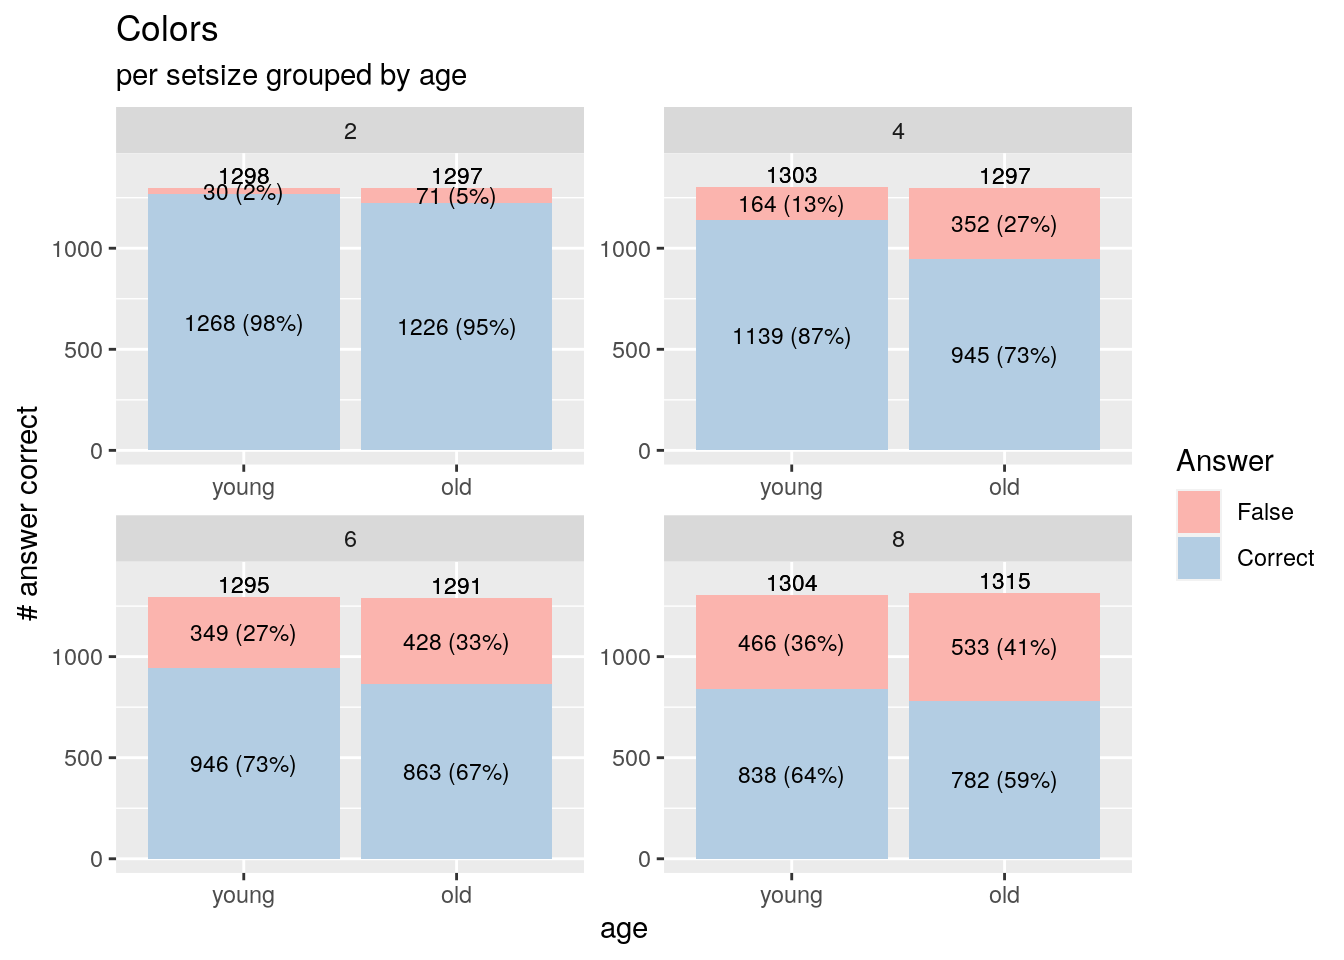
\includegraphics{CvsRW_files/figure-latex/unnamed-chunk-7-1.pdf}

\begin{Shaded}
\begin{Highlighting}[]
\NormalTok{objectList }\OperatorTok\StringTok{ }\KeywordTok{mutate}\NormalTok{(}\DataTypeTok{age=}\KeywordTok{factor}\NormalTok{(age, }\DataTypeTok{levels =} \KeywordTok{c}\NormalTok{(}\StringTok{"young"}\NormalTok{,}\StringTok{"old"}\NormalTok{)),}
             \DataTypeTok{answer_correct=}\KeywordTok{factor}\NormalTok{(answer_correct, }\DataTypeTok{levels =} \KeywordTok{c}\NormalTok{(}\DecValTok{0}\NormalTok{,}\DecValTok{1}\NormalTok{),}\DataTypeTok{labels =} \KeywordTok{c}\NormalTok{(}\StringTok{"False"}\NormalTok{,}\StringTok{"Correct"}\NormalTok{))) }\OperatorTok
\StringTok{  }\KeywordTok{group_by}\NormalTok{(age,setsize,answer_correct) }\OperatorTok\StringTok{ }\KeywordTok{summarise}\NormalTok{(}\DataTypeTok{N=}\KeywordTok{n}\NormalTok{()) }\OperatorTok\StringTok{ }\KeywordTok{ungroup}\NormalTok{() }\OperatorTok
\StringTok{  }\KeywordTok{group_by}\NormalTok{(age,setsize) }\OperatorTok\StringTok{ }
\StringTok{  }\KeywordTok{mutate}\NormalTok{(}\DataTypeTok{Total=}\KeywordTok{sum}\NormalTok{(N),}\DataTypeTok{Percent=}\NormalTok{N}\OperatorTok{/}\NormalTok{Total,}
         \DataTypeTok{Lab=}\KeywordTok{paste0}\NormalTok{(N,}\StringTok{' ('}\NormalTok{,}\KeywordTok{paste0}\NormalTok{(}\KeywordTok{round}\NormalTok{(}\DecValTok{100}\OperatorTok{*}\NormalTok{Percent,}\DecValTok{0}\NormalTok{),}\StringTok{'%'}\NormalTok{),}\StringTok{')'}\NormalTok{)) ->}\StringTok{ }\NormalTok{SumsObjects}
\end{Highlighting}
\end{Shaded}

\begin{verbatim}
## `summarise()` regrouping output by 'age', 'setsize' (override with `.groups` argument)
\end{verbatim}

\begin{Shaded}
\begin{Highlighting}[]
\CommentTok{#Plot}
\KeywordTok{ggplot}\NormalTok{(SumsObjects,}\KeywordTok{aes}\NormalTok{(}\DataTypeTok{x=}\NormalTok{age,}\DataTypeTok{y=}\NormalTok{N,}\DataTypeTok{fill=}\NormalTok{answer_correct))}\OperatorTok{+}
\StringTok{  }\KeywordTok{geom_bar}\NormalTok{(}\DataTypeTok{stat=}\StringTok{'identity'}\NormalTok{,}\DataTypeTok{position =} \KeywordTok{position_stack}\NormalTok{())}\OperatorTok{+}
\StringTok{  }\KeywordTok{facet_wrap}\NormalTok{(.}\OperatorTok{~}\NormalTok{setsize,}\DataTypeTok{scales =} \StringTok{'free'}\NormalTok{)}\OperatorTok{+}
\StringTok{  }\KeywordTok{geom_text}\NormalTok{(}\KeywordTok{aes}\NormalTok{(}\DataTypeTok{label=}\NormalTok{Lab),}\DataTypeTok{position =} \KeywordTok{position_stack}\NormalTok{(}\DataTypeTok{vjust =} \FloatTok{.5}\NormalTok{),}\DataTypeTok{size=}\DecValTok{3}\NormalTok{)}\OperatorTok{+}
\StringTok{  }\KeywordTok{geom_text}\NormalTok{(}\KeywordTok{aes}\NormalTok{(}\DataTypeTok{y=}\NormalTok{Total,}\DataTypeTok{label=}\NormalTok{Total),}\DataTypeTok{vjust=}\OperatorTok{-}\FloatTok{0.25}\NormalTok{,}\DataTypeTok{size=}\DecValTok{3}\NormalTok{)}\OperatorTok{+}
\StringTok{  }\KeywordTok{labs}\NormalTok{(}\DataTypeTok{title=}\StringTok{"Real world objects"}\NormalTok{,}\DataTypeTok{subtitle =} \StringTok{"per setsize grouped by age"}\NormalTok{, }\DataTypeTok{x=}\StringTok{"age"}\NormalTok{, }\DataTypeTok{y=}\StringTok{"# answer correct"}\NormalTok{, }\DataTypeTok{fill=}\StringTok{"Answer"}\NormalTok{)}\OperatorTok{+}\KeywordTok{scale_fill_brewer}\NormalTok{(}\DataTypeTok{palette =} \StringTok{"Pastel1"}\NormalTok{)}
\end{Highlighting}
\end{Shaded}

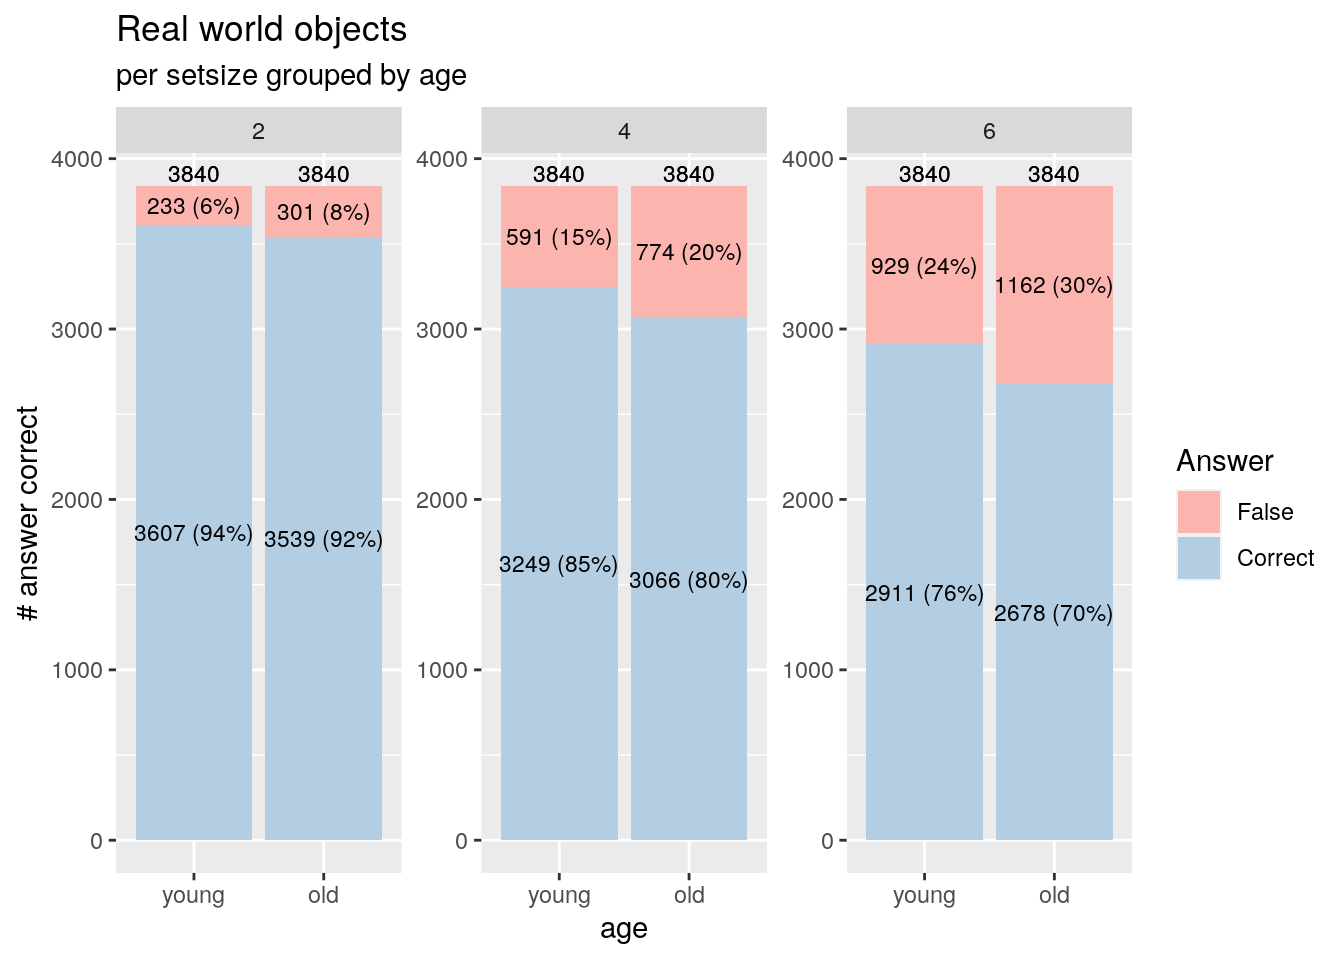
\includegraphics{CvsRW_files/figure-latex/unnamed-chunk-7-2.pdf} Plotte
die Streuung von Colors und real objects

\begin{Shaded}
\begin{Highlighting}[]
\NormalTok{colorListResult }\OperatorTok\StringTok{  }\KeywordTok{ggplot}\NormalTok{(}\DataTypeTok{mapping=}\KeywordTok{aes}\NormalTok{(}\DataTypeTok{x=}\NormalTok{age, }\DataTypeTok{y=}\NormalTok{mean_answer_correct,}\DataTypeTok{fill=}\NormalTok{age)) }\OperatorTok{+}\StringTok{ }\KeywordTok{geom_violin}\NormalTok{() }\OperatorTok{+}\StringTok{ }\KeywordTok{geom_jitter}\NormalTok{(}\DataTypeTok{width =} \FloatTok{0.2}\NormalTok{, }\DataTypeTok{alpha =} \FloatTok{0.6}\NormalTok{)}\OperatorTok{+}\KeywordTok{scale_y_continuous}\NormalTok{(}\DataTypeTok{labels =}\NormalTok{ scales}\OperatorTok{::}\NormalTok{percent)}\OperatorTok{+}\KeywordTok{labs}\NormalTok{(}\DataTypeTok{title=}\StringTok{"Colors"}\NormalTok{,}\DataTypeTok{subtitle =} \StringTok{"distribution test persons mean value of correct answers"}\NormalTok{, }\DataTypeTok{x=}\StringTok{"age"}\NormalTok{, }\DataTypeTok{y=}\StringTok{"mean answers correct"}\NormalTok{, }\DataTypeTok{fill=}\StringTok{"Answer"}\NormalTok{)}
\end{Highlighting}
\end{Shaded}

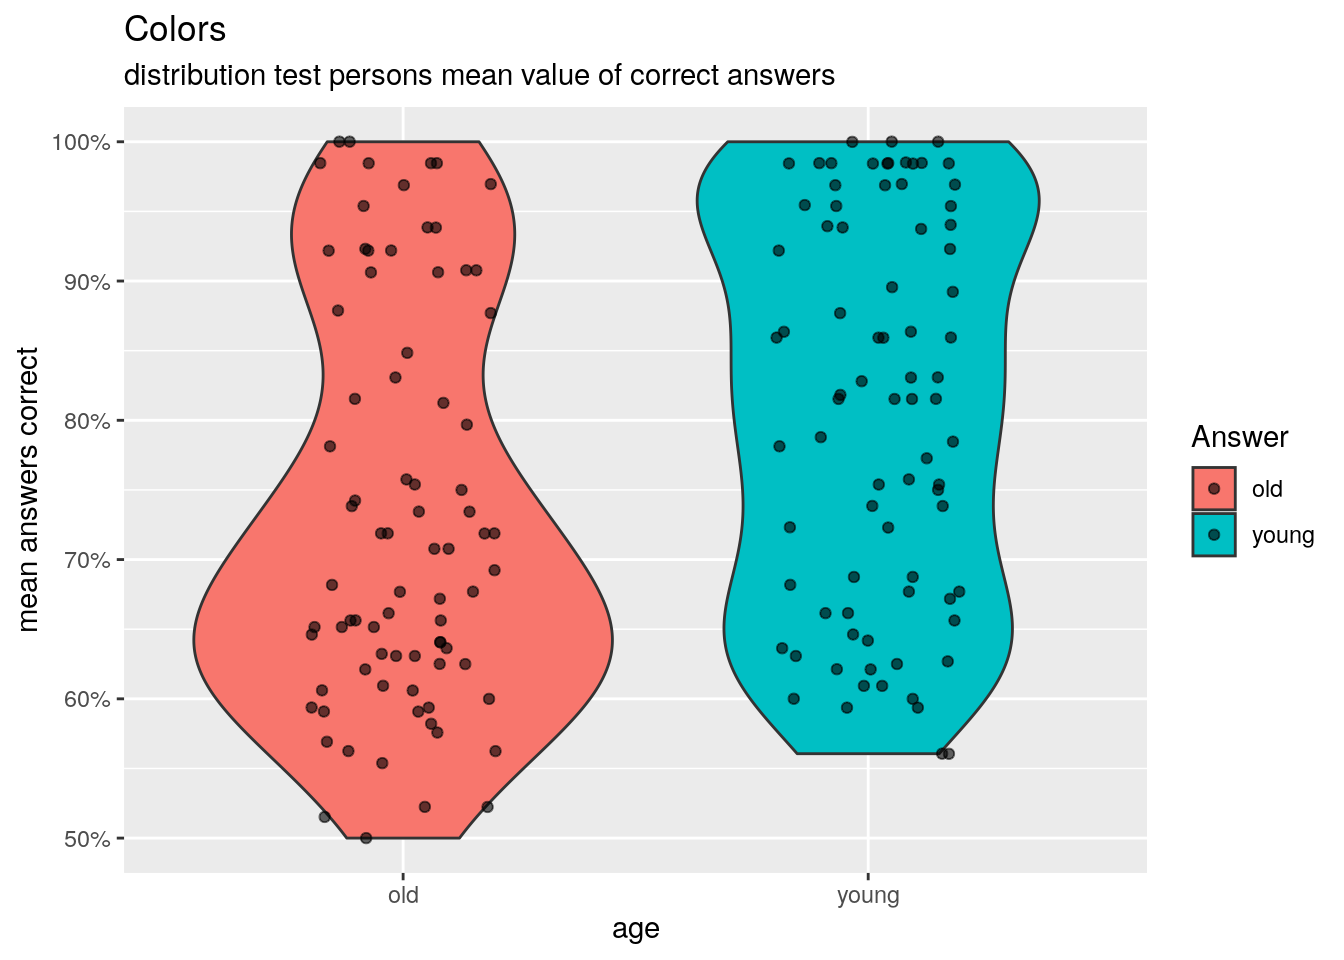
\includegraphics{CvsRW_files/figure-latex/unnamed-chunk-8-1.pdf}

\begin{Shaded}
\begin{Highlighting}[]
\NormalTok{objectResult }\OperatorTok\StringTok{  }\KeywordTok{ggplot}\NormalTok{(}\DataTypeTok{mapping=}\KeywordTok{aes}\NormalTok{(}\DataTypeTok{x=}\NormalTok{age, }\DataTypeTok{y=}\NormalTok{mean_answer_correct,}\DataTypeTok{fill=}\NormalTok{age)) }\OperatorTok{+}\StringTok{ }\KeywordTok{geom_violin}\NormalTok{() }\OperatorTok{+}\StringTok{ }\KeywordTok{geom_jitter}\NormalTok{(}\DataTypeTok{width =} \FloatTok{0.2}\NormalTok{, }\DataTypeTok{alpha =} \FloatTok{0.6}\NormalTok{)}\OperatorTok{+}\KeywordTok{scale_y_continuous}\NormalTok{(}\DataTypeTok{labels =}\NormalTok{ scales}\OperatorTok{::}\NormalTok{percent)}\OperatorTok{+}\KeywordTok{labs}\NormalTok{(}\DataTypeTok{title=}\StringTok{"Real world objects"}\NormalTok{,}\DataTypeTok{subtitle =} \StringTok{"distribution test persons mean value of correct answers"}\NormalTok{, }\DataTypeTok{x=}\StringTok{"age"}\NormalTok{, }\DataTypeTok{y=}\StringTok{"mean answers correct"}\NormalTok{, }\DataTypeTok{fill=}\StringTok{"Answer"}\NormalTok{)}
\end{Highlighting}
\end{Shaded}

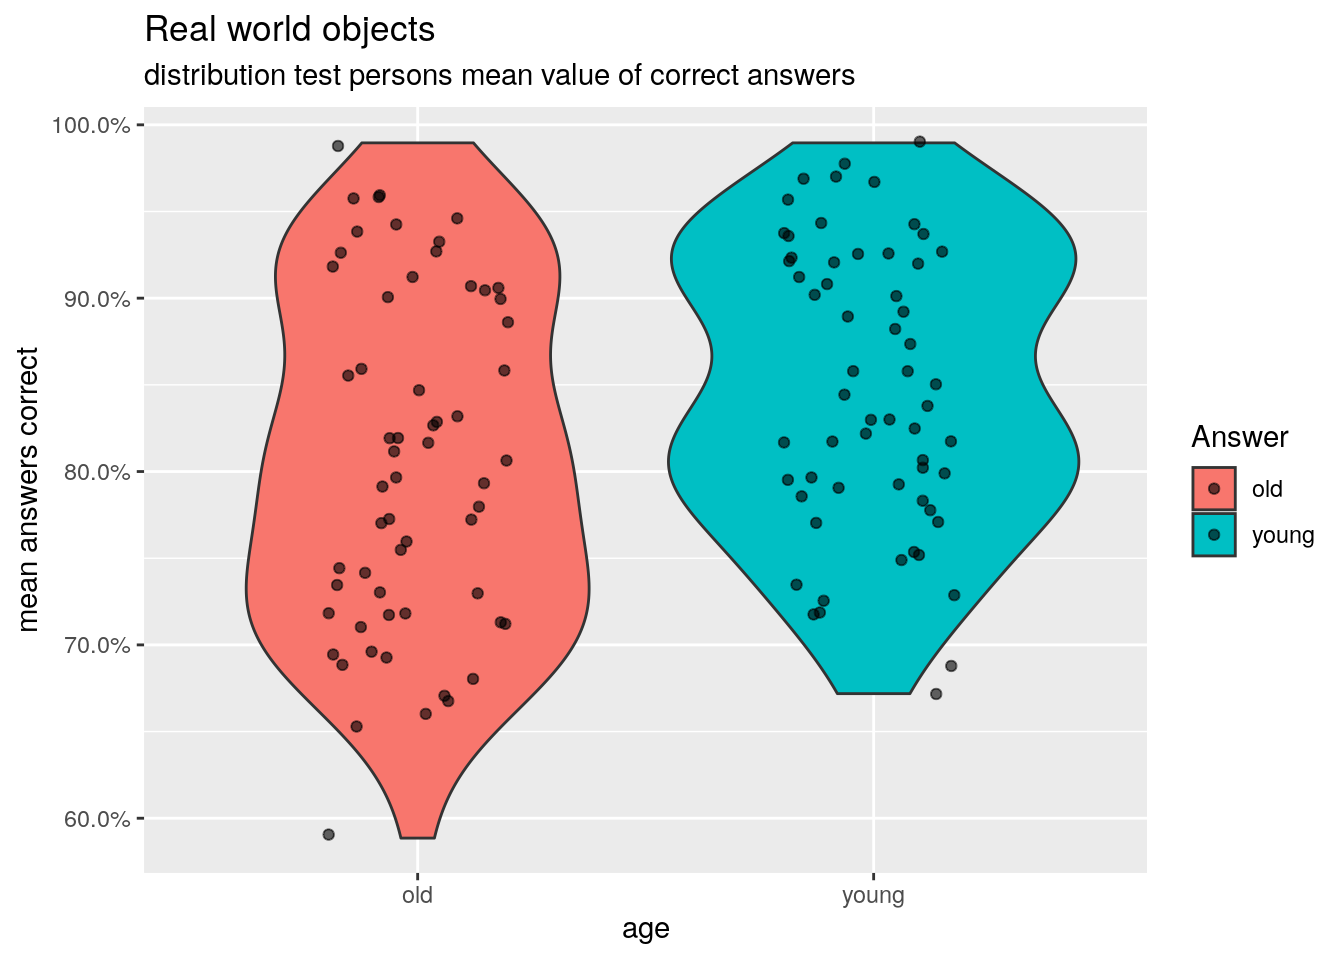
\includegraphics{CvsRW_files/figure-latex/unnamed-chunk-8-2.pdf}

\begin{Shaded}
\begin{Highlighting}[]
\NormalTok{colorListResult }\OperatorTok\StringTok{  }\KeywordTok{ggplot}\NormalTok{(}\DataTypeTok{mapping=}\KeywordTok{aes}\NormalTok{(}\DataTypeTok{x=}\NormalTok{age, }\DataTypeTok{y=}\NormalTok{mean_answer_correct,}\DataTypeTok{fill=}\NormalTok{age))}\OperatorTok{+}\StringTok{ }\KeywordTok{geom_violin}\NormalTok{() }\OperatorTok{+}\StringTok{ }\KeywordTok{geom_jitter}\NormalTok{(}\DataTypeTok{width =} \FloatTok{0.2}\NormalTok{, }\DataTypeTok{alpha =} \FloatTok{0.6}\NormalTok{)}\OperatorTok{+}\KeywordTok{facet_wrap}\NormalTok{(.}\OperatorTok{~}\NormalTok{condition,}\DataTypeTok{scales =} \StringTok{'free'}\NormalTok{)}\OperatorTok{+}\KeywordTok{scale_y_continuous}\NormalTok{(}\DataTypeTok{labels =}\NormalTok{ scales}\OperatorTok{::}\NormalTok{percent)}\OperatorTok{+}\KeywordTok{labs}\NormalTok{(}\DataTypeTok{title=}\StringTok{"Colors"}\NormalTok{,}\DataTypeTok{subtitle =} \StringTok{"distribution test persons mean value of correct answers"}\NormalTok{, }\DataTypeTok{x=}\StringTok{"age"}\NormalTok{, }\DataTypeTok{y=}\StringTok{"mean answers correct"}\NormalTok{, }\DataTypeTok{fill=}\StringTok{"Answer"}\NormalTok{)}
\end{Highlighting}
\end{Shaded}

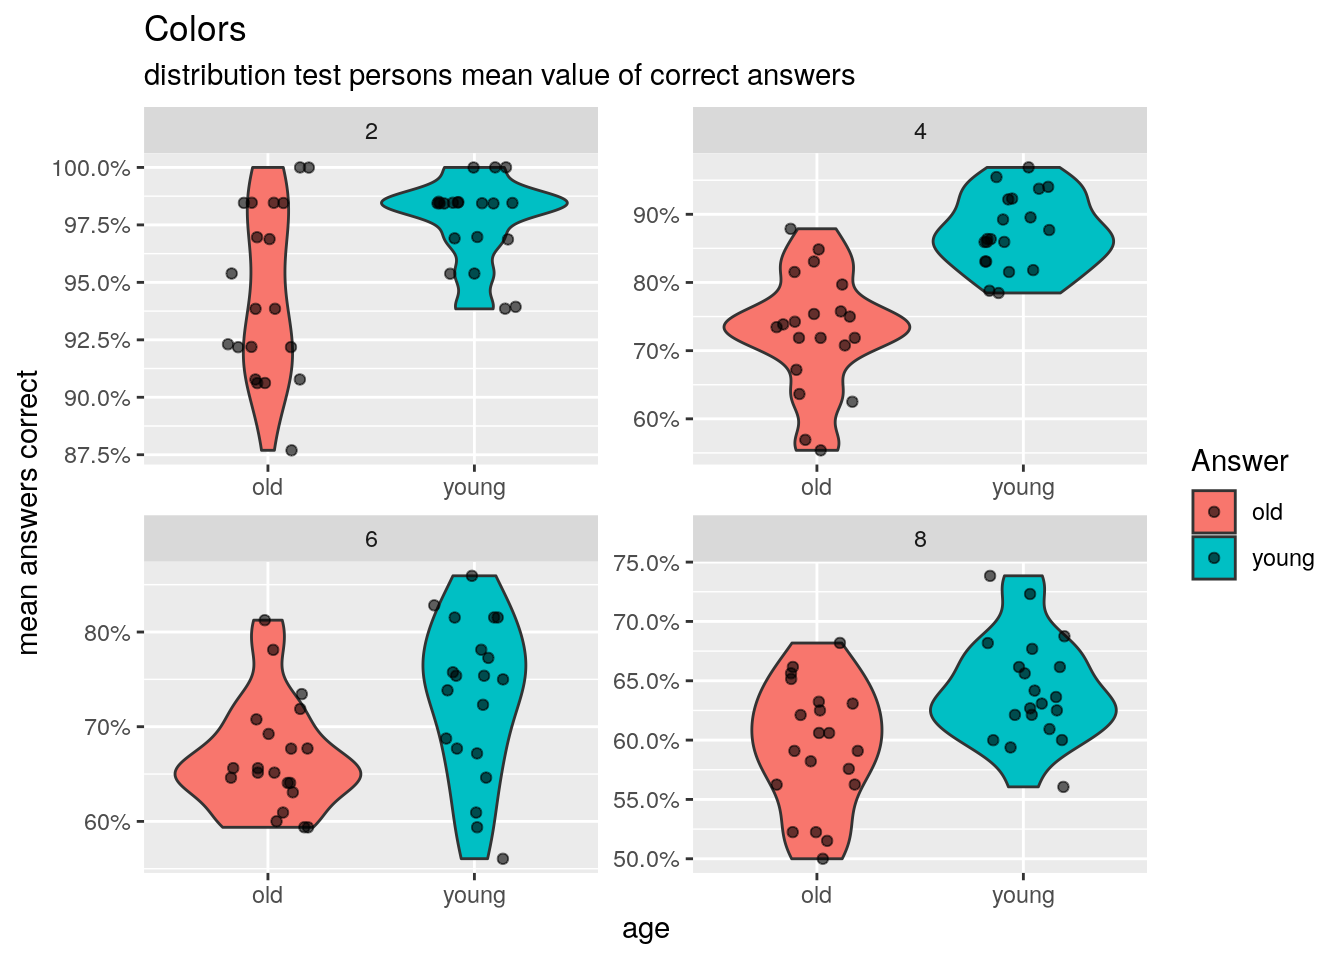
\includegraphics{CvsRW_files/figure-latex/unnamed-chunk-8-3.pdf}

\begin{Shaded}
\begin{Highlighting}[]
\NormalTok{objectResult }\OperatorTok\StringTok{  }\KeywordTok{ggplot}\NormalTok{(}\DataTypeTok{mapping=}\KeywordTok{aes}\NormalTok{(}\DataTypeTok{x=}\NormalTok{age, }\DataTypeTok{y=}\NormalTok{mean_answer_correct,}\DataTypeTok{fill=}\NormalTok{age))}\OperatorTok{+}\StringTok{ }\KeywordTok{geom_violin}\NormalTok{() }\OperatorTok{+}\StringTok{ }\KeywordTok{geom_jitter}\NormalTok{(}\DataTypeTok{width =} \FloatTok{0.2}\NormalTok{, }\DataTypeTok{alpha =} \FloatTok{0.6}\NormalTok{)}\OperatorTok{+}\KeywordTok{facet_wrap}\NormalTok{(.}\OperatorTok{~}\NormalTok{setsize,}\DataTypeTok{scales =} \StringTok{'free'}\NormalTok{)}\OperatorTok{+}\KeywordTok{scale_y_continuous}\NormalTok{(}\DataTypeTok{labels =}\NormalTok{ scales}\OperatorTok{::}\NormalTok{percent)}\OperatorTok{+}\KeywordTok{labs}\NormalTok{(}\DataTypeTok{title=}\StringTok{"Real world objects"}\NormalTok{,}\DataTypeTok{subtitle =} \StringTok{"distribution test persons mean value of correct answers"}\NormalTok{, }\DataTypeTok{x=}\StringTok{"age"}\NormalTok{, }\DataTypeTok{y=}\StringTok{"mean answers correct"}\NormalTok{, }\DataTypeTok{fill=}\StringTok{"Answer"}\NormalTok{)}
\end{Highlighting}
\end{Shaded}

\includegraphics{CvsRW_files/figure-latex/unnamed-chunk-8-4.pdf}

\begin{Shaded}
\begin{Highlighting}[]
\NormalTok{colorListResult }\OperatorTok\StringTok{  }\KeywordTok{ggplot}\NormalTok{(}\DataTypeTok{mapping=}\KeywordTok{aes}\NormalTok{(}\DataTypeTok{x=}\NormalTok{age, }\DataTypeTok{y=}\NormalTok{mean_answer_correct,}\DataTypeTok{fill=}\NormalTok{age)) }\OperatorTok{+}\StringTok{ }\KeywordTok{geom_boxplot}\NormalTok{() }\OperatorTok{+}\StringTok{ }\KeywordTok{geom_jitter}\NormalTok{(}\DataTypeTok{width =} \FloatTok{0.2}\NormalTok{, }\DataTypeTok{alpha =} \FloatTok{0.6}\NormalTok{)}\OperatorTok{+}\KeywordTok{scale_y_continuous}\NormalTok{(}\DataTypeTok{labels =}\NormalTok{ scales}\OperatorTok{::}\NormalTok{percent)}\OperatorTok{+}\KeywordTok{labs}\NormalTok{(}\DataTypeTok{title=}\StringTok{"Colors"}\NormalTok{,}\DataTypeTok{subtitle =} \StringTok{"distribution test persons mean value of correct answers"}\NormalTok{, }\DataTypeTok{x=}\StringTok{"age"}\NormalTok{, }\DataTypeTok{y=}\StringTok{"mean answers correct"}\NormalTok{, }\DataTypeTok{fill=}\StringTok{"Answer"}\NormalTok{)}
\end{Highlighting}
\end{Shaded}

\includegraphics{CvsRW_files/figure-latex/unnamed-chunk-8-5.pdf}

\begin{Shaded}
\begin{Highlighting}[]
\NormalTok{objectResult }\OperatorTok\StringTok{  }\KeywordTok{ggplot}\NormalTok{(}\DataTypeTok{mapping=}\KeywordTok{aes}\NormalTok{(}\DataTypeTok{x=}\NormalTok{age, }\DataTypeTok{y=}\NormalTok{mean_answer_correct,}\DataTypeTok{fill=}\NormalTok{age)) }\OperatorTok{+}\StringTok{ }\KeywordTok{geom_boxplot}\NormalTok{() }\OperatorTok{+}\StringTok{ }\KeywordTok{geom_jitter}\NormalTok{(}\DataTypeTok{width =} \FloatTok{0.2}\NormalTok{, }\DataTypeTok{alpha =} \FloatTok{0.6}\NormalTok{)}\OperatorTok{+}\KeywordTok{scale_y_continuous}\NormalTok{(}\DataTypeTok{labels =}\NormalTok{ scales}\OperatorTok{::}\NormalTok{percent)}\OperatorTok{+}\KeywordTok{labs}\NormalTok{(}\DataTypeTok{title=}\StringTok{"Real world objects"}\NormalTok{,}\DataTypeTok{subtitle =} \StringTok{"distribution test persons mean value of correct answers"}\NormalTok{, }\DataTypeTok{x=}\StringTok{"age"}\NormalTok{, }\DataTypeTok{y=}\StringTok{"mean answers correct"}\NormalTok{, }\DataTypeTok{fill=}\StringTok{"Answer"}\NormalTok{)}
\end{Highlighting}
\end{Shaded}

\includegraphics{CvsRW_files/figure-latex/unnamed-chunk-8-6.pdf}

\begin{Shaded}
\begin{Highlighting}[]
\NormalTok{colorListResult }\OperatorTok\StringTok{  }\KeywordTok{ggplot}\NormalTok{(}\DataTypeTok{mapping=}\KeywordTok{aes}\NormalTok{(}\DataTypeTok{x=}\NormalTok{age, }\DataTypeTok{y=}\NormalTok{mean_answer_correct,}\DataTypeTok{fill=}\NormalTok{age))}\OperatorTok{+}\StringTok{ }\KeywordTok{geom_boxplot}\NormalTok{() }\OperatorTok{+}\StringTok{ }\KeywordTok{geom_jitter}\NormalTok{(}\DataTypeTok{width =} \FloatTok{0.2}\NormalTok{, }\DataTypeTok{alpha =} \FloatTok{0.6}\NormalTok{)}\OperatorTok{+}\KeywordTok{facet_wrap}\NormalTok{(.}\OperatorTok{~}\NormalTok{condition,}\DataTypeTok{scales =} \StringTok{'free'}\NormalTok{)}\OperatorTok{+}\KeywordTok{scale_y_continuous}\NormalTok{(}\DataTypeTok{labels =}\NormalTok{ scales}\OperatorTok{::}\NormalTok{percent)}\OperatorTok{+}\KeywordTok{labs}\NormalTok{(}\DataTypeTok{title=}\StringTok{"Colors"}\NormalTok{,}\DataTypeTok{subtitle =} \StringTok{"distribution test persons mean value of correct answers"}\NormalTok{, }\DataTypeTok{x=}\StringTok{"age"}\NormalTok{, }\DataTypeTok{y=}\StringTok{"mean answers correct"}\NormalTok{, }\DataTypeTok{fill=}\StringTok{"Answer"}\NormalTok{)}
\end{Highlighting}
\end{Shaded}

\includegraphics{CvsRW_files/figure-latex/unnamed-chunk-8-7.pdf}

\begin{Shaded}
\begin{Highlighting}[]
\NormalTok{objectResult }\OperatorTok\StringTok{  }\KeywordTok{ggplot}\NormalTok{(}\DataTypeTok{mapping=}\KeywordTok{aes}\NormalTok{(}\DataTypeTok{x=}\NormalTok{age, }\DataTypeTok{y=}\NormalTok{mean_answer_correct,}\DataTypeTok{fill=}\NormalTok{age))}\OperatorTok{+}\StringTok{ }\KeywordTok{geom_boxplot}\NormalTok{() }\OperatorTok{+}\StringTok{ }\KeywordTok{geom_jitter}\NormalTok{(}\DataTypeTok{width =} \FloatTok{0.2}\NormalTok{, }\DataTypeTok{alpha =} \FloatTok{0.6}\NormalTok{)}\OperatorTok{+}\KeywordTok{facet_wrap}\NormalTok{(.}\OperatorTok{~}\NormalTok{setsize,}\DataTypeTok{scales =} \StringTok{'free'}\NormalTok{)}\OperatorTok{+}\KeywordTok{scale_y_continuous}\NormalTok{(}\DataTypeTok{labels =}\NormalTok{ scales}\OperatorTok{::}\NormalTok{percent)}\OperatorTok{+}\KeywordTok{labs}\NormalTok{(}\DataTypeTok{title=}\StringTok{"Real world objects"}\NormalTok{,}\DataTypeTok{subtitle =} \StringTok{"distribution test persons mean value of correct answers"}\NormalTok{, }\DataTypeTok{x=}\StringTok{"age"}\NormalTok{, }\DataTypeTok{y=}\StringTok{"mean answers correct"}\NormalTok{, }\DataTypeTok{fill=}\StringTok{"Answer"}\NormalTok{)}
\end{Highlighting}
\end{Shaded}

\includegraphics{CvsRW_files/figure-latex/unnamed-chunk-8-8.pdf}

Häufigkeitsverteilung

\begin{Shaded}
\begin{Highlighting}[]
\NormalTok{colorListResult }\OperatorTok\StringTok{  }\KeywordTok{ggplot}\NormalTok{(}\DataTypeTok{mapping=}\KeywordTok{aes}\NormalTok{(}\DataTypeTok{x=}\NormalTok{mean_answer_correct, }\DataTypeTok{fill=}\NormalTok{age))}\OperatorTok{+}\StringTok{ }\KeywordTok{geom_histogram}\NormalTok{(}\DataTypeTok{bins =} \DecValTok{20}\NormalTok{)}\OperatorTok{+}\KeywordTok{labs}\NormalTok{(}\DataTypeTok{title=}\StringTok{"Colors"}\NormalTok{,}\DataTypeTok{subtitle =} \StringTok{"Häufigkeiten korrekter Antworten"}\NormalTok{, }\DataTypeTok{x=}\StringTok{"Mean answers correct"}\NormalTok{)}\OperatorTok{+}\KeywordTok{scale_x_continuous}\NormalTok{(}\DataTypeTok{labels =}\NormalTok{ scales}\OperatorTok{::}\NormalTok{percent)}
\end{Highlighting}
\end{Shaded}

\includegraphics{CvsRW_files/figure-latex/unnamed-chunk-9-1.pdf}

\begin{Shaded}
\begin{Highlighting}[]
\NormalTok{colorListResult }\OperatorTok\StringTok{  }\KeywordTok{ggplot}\NormalTok{(}\DataTypeTok{mapping=}\KeywordTok{aes}\NormalTok{(}\DataTypeTok{x=}\NormalTok{mean_answer_correct, }\DataTypeTok{fill=}\NormalTok{age))}\OperatorTok{+}\StringTok{ }\KeywordTok{geom_histogram}\NormalTok{(}\DataTypeTok{bins=}\DecValTok{20}\NormalTok{)}\OperatorTok{+}\KeywordTok{facet_wrap}\NormalTok{(.}\OperatorTok{~}\NormalTok{condition,}\DataTypeTok{scales =} \StringTok{'free'}\NormalTok{)}\OperatorTok{+}\KeywordTok{scale_x_continuous}\NormalTok{(}\DataTypeTok{labels =}\NormalTok{ scales}\OperatorTok{::}\NormalTok{percent)}\OperatorTok{+}\KeywordTok{labs}\NormalTok{(}\DataTypeTok{title=}\StringTok{"Colors"}\NormalTok{,}\DataTypeTok{subtitle =} \StringTok{"Häufigkeiten korrekter Antworten"}\NormalTok{, }\DataTypeTok{x=}\StringTok{"Mean answers correct"}\NormalTok{)}
\end{Highlighting}
\end{Shaded}

\includegraphics{CvsRW_files/figure-latex/unnamed-chunk-9-2.pdf}

\begin{Shaded}
\begin{Highlighting}[]
\NormalTok{objectResult }\OperatorTok\StringTok{  }\KeywordTok{ggplot}\NormalTok{(}\DataTypeTok{mapping=}\KeywordTok{aes}\NormalTok{(}\DataTypeTok{x=}\NormalTok{mean_answer_correct, }\DataTypeTok{fill=}\NormalTok{age))}\OperatorTok{+}\StringTok{ }\KeywordTok{geom_histogram}\NormalTok{(}\DataTypeTok{bins=}\DecValTok{20}\NormalTok{)}\OperatorTok{+}\KeywordTok{labs}\NormalTok{(}\DataTypeTok{title=}\StringTok{"Real world objects"}\NormalTok{,}\DataTypeTok{subtitle =} \StringTok{"Häufigkeiten korrekter Antworten"}\NormalTok{, }\DataTypeTok{x=}\StringTok{"Mean answers correct"}\NormalTok{)}\OperatorTok{+}\KeywordTok{scale_x_continuous}\NormalTok{(}\DataTypeTok{labels =}\NormalTok{ scales}\OperatorTok{::}\NormalTok{percent)}
\end{Highlighting}
\end{Shaded}

\includegraphics{CvsRW_files/figure-latex/unnamed-chunk-9-3.pdf}

\begin{Shaded}
\begin{Highlighting}[]
\NormalTok{objectResult }\OperatorTok\StringTok{  }\KeywordTok{ggplot}\NormalTok{(}\DataTypeTok{mapping=}\KeywordTok{aes}\NormalTok{(}\DataTypeTok{x=}\NormalTok{mean_answer_correct, }\DataTypeTok{fill=}\NormalTok{age))}\OperatorTok{+}\StringTok{ }\KeywordTok{geom_histogram}\NormalTok{(}\DataTypeTok{bins=}\DecValTok{20}\NormalTok{)}\OperatorTok{+}\KeywordTok{facet_wrap}\NormalTok{(.}\OperatorTok{~}\NormalTok{setsize,}\DataTypeTok{scales =} \StringTok{'free'}\NormalTok{)}\OperatorTok{+}\KeywordTok{scale_x_continuous}\NormalTok{(}\DataTypeTok{labels =}\NormalTok{ scales}\OperatorTok{::}\NormalTok{percent)}\OperatorTok{+}\KeywordTok{labs}\NormalTok{(}\DataTypeTok{title=}\StringTok{"Real world objects"}\NormalTok{,}\DataTypeTok{subtitle =} \StringTok{"Häufigkeiten korrekter Antworten"}\NormalTok{, }\DataTypeTok{x=}\StringTok{"Mean answers correct"}\NormalTok{)}
\end{Highlighting}
\end{Shaded}

\includegraphics{CvsRW_files/figure-latex/unnamed-chunk-9-4.pdf}

\begin{Shaded}
\begin{Highlighting}[]
\NormalTok{colorListResult }\OperatorTok\StringTok{  }\KeywordTok{ggplot}\NormalTok{(}\DataTypeTok{mapping=}\KeywordTok{aes}\NormalTok{(}\DataTypeTok{x=}\NormalTok{mean_answer_correct, }\DataTypeTok{fill=}\NormalTok{age))}\OperatorTok{+}\StringTok{ }\KeywordTok{geom_density}\NormalTok{ (}\DataTypeTok{alpha=}\FloatTok{0.2}\NormalTok{)}\OperatorTok{+}\KeywordTok{labs}\NormalTok{(}\DataTypeTok{title=}\StringTok{"Colors"}\NormalTok{,}\DataTypeTok{subtitle =} \StringTok{"Häufigkeiten korrekter Antworten"}\NormalTok{, }\DataTypeTok{x=}\StringTok{"Mean answers correct"}\NormalTok{)}\OperatorTok{+}\KeywordTok{scale_x_continuous}\NormalTok{(}\DataTypeTok{labels =}\NormalTok{ scales}\OperatorTok{::}\NormalTok{percent)}
\end{Highlighting}
\end{Shaded}

\includegraphics{CvsRW_files/figure-latex/unnamed-chunk-9-5.pdf}

\begin{Shaded}
\begin{Highlighting}[]
\NormalTok{colorListResult }\OperatorTok\StringTok{  }\KeywordTok{ggplot}\NormalTok{(}\DataTypeTok{mapping=}\KeywordTok{aes}\NormalTok{(}\DataTypeTok{x=}\NormalTok{mean_answer_correct, }\DataTypeTok{fill=}\NormalTok{age))}\OperatorTok{+}\StringTok{ }\KeywordTok{geom_density}\NormalTok{( }\DataTypeTok{alpha=}\FloatTok{0.2}\NormalTok{)}\OperatorTok{+}\KeywordTok{facet_wrap}\NormalTok{(.}\OperatorTok{~}\NormalTok{condition,}\DataTypeTok{scales =} \StringTok{'free'}\NormalTok{)}\OperatorTok{+}\KeywordTok{scale_x_continuous}\NormalTok{(}\DataTypeTok{labels =}\NormalTok{ scales}\OperatorTok{::}\NormalTok{percent)}\OperatorTok{+}\KeywordTok{labs}\NormalTok{(}\DataTypeTok{title=}\StringTok{"Colors"}\NormalTok{,}\DataTypeTok{subtitle =} \StringTok{"Häufigkeiten korrekter Antworten"}\NormalTok{, }\DataTypeTok{x=}\StringTok{"Mean answers correct"}\NormalTok{)}
\end{Highlighting}
\end{Shaded}

\includegraphics{CvsRW_files/figure-latex/unnamed-chunk-9-6.pdf}

\begin{Shaded}
\begin{Highlighting}[]
\NormalTok{objectResult }\OperatorTok\StringTok{  }\KeywordTok{ggplot}\NormalTok{(}\DataTypeTok{mapping=}\KeywordTok{aes}\NormalTok{(}\DataTypeTok{x=}\NormalTok{mean_answer_correct, }\DataTypeTok{fill=}\NormalTok{age))}\OperatorTok{+}\StringTok{ }\KeywordTok{geom_density}\NormalTok{(}\DataTypeTok{alpha=}\FloatTok{0.2}\NormalTok{)}\OperatorTok{+}\KeywordTok{labs}\NormalTok{(}\DataTypeTok{title=}\StringTok{"Real world objects"}\NormalTok{,}\DataTypeTok{subtitle =} \StringTok{"Häufigkeiten korrekter Antworten"}\NormalTok{, }\DataTypeTok{x=}\StringTok{"Mean answers correct"}\NormalTok{)}\OperatorTok{+}\KeywordTok{scale_x_continuous}\NormalTok{(}\DataTypeTok{labels =}\NormalTok{ scales}\OperatorTok{::}\NormalTok{percent)}
\end{Highlighting}
\end{Shaded}

\includegraphics{CvsRW_files/figure-latex/unnamed-chunk-9-7.pdf}

\begin{Shaded}
\begin{Highlighting}[]
\NormalTok{objectResult }\OperatorTok\StringTok{  }\KeywordTok{ggplot}\NormalTok{(}\DataTypeTok{mapping=}\KeywordTok{aes}\NormalTok{(}\DataTypeTok{x=}\NormalTok{mean_answer_correct, }\DataTypeTok{fill=}\NormalTok{age))}\OperatorTok{+}\StringTok{ }\KeywordTok{geom_density}\NormalTok{(}\DataTypeTok{alpha=}\FloatTok{0.2}\NormalTok{)}\OperatorTok{+}\KeywordTok{facet_wrap}\NormalTok{(.}\OperatorTok{~}\NormalTok{setsize,}\DataTypeTok{scales =} \StringTok{'free'}\NormalTok{)}\OperatorTok{+}\KeywordTok{scale_x_continuous}\NormalTok{(}\DataTypeTok{labels =}\NormalTok{ scales}\OperatorTok{::}\NormalTok{percent)}\OperatorTok{+}\KeywordTok{labs}\NormalTok{(}\DataTypeTok{title=}\StringTok{"Real world objects"}\NormalTok{,}\DataTypeTok{subtitle =} \StringTok{"Häufigkeiten korrekter Antworten"}\NormalTok{, }\DataTypeTok{x=}\StringTok{"Mean answers correct"}\NormalTok{)}
\end{Highlighting}
\end{Shaded}

\includegraphics{CvsRW_files/figure-latex/unnamed-chunk-9-8.pdf}
Vergleich Color vs.~Objects gleiche Altersgruppen

\begin{Shaded}
\begin{Highlighting}[]
\NormalTok{joinedTestList }\OperatorTok\StringTok{  }\KeywordTok{ggplot}\NormalTok{(}\DataTypeTok{mapping=}\KeywordTok{aes}\NormalTok{(}\DataTypeTok{x=}\NormalTok{mean_answer_correct, }\DataTypeTok{fill=}\NormalTok{test))}\OperatorTok{+}\StringTok{ }\KeywordTok{geom_density}\NormalTok{ (}\DataTypeTok{alpha=}\FloatTok{0.2}\NormalTok{)}\OperatorTok{+}\KeywordTok{labs}\NormalTok{(}\DataTypeTok{title=}\StringTok{"Colors vs Object"}\NormalTok{,}\DataTypeTok{subtitle =} \StringTok{"Häufigkeiten korrekter Antworten"}\NormalTok{, }\DataTypeTok{x=}\StringTok{"Mean answers correct"}\NormalTok{)}\OperatorTok{+}\KeywordTok{scale_x_continuous}\NormalTok{(}\DataTypeTok{labels =}\NormalTok{ scales}\OperatorTok{::}\NormalTok{percent)}
\end{Highlighting}
\end{Shaded}

\includegraphics{CvsRW_files/figure-latex/unnamed-chunk-10-1.pdf}

\begin{Shaded}
\begin{Highlighting}[]
\NormalTok{joinedTestList }\OperatorTok\StringTok{  }\KeywordTok{ggplot}\NormalTok{(}\DataTypeTok{mapping=}\KeywordTok{aes}\NormalTok{(}\DataTypeTok{x=}\NormalTok{mean_answer_correct, }\DataTypeTok{fill=}\NormalTok{test))}\OperatorTok{+}\StringTok{ }\KeywordTok{geom_density}\NormalTok{ (}\DataTypeTok{alpha=}\FloatTok{0.2}\NormalTok{)}\OperatorTok{+}\KeywordTok{facet_wrap}\NormalTok{(.}\OperatorTok{~}\NormalTok{setsize,}\DataTypeTok{scales =} \StringTok{'free'}\NormalTok{)}\OperatorTok{+}\KeywordTok{labs}\NormalTok{(}\DataTypeTok{title=}\StringTok{"Colors vs Object"}\NormalTok{,}\DataTypeTok{subtitle =} \StringTok{"Häufigkeiten korrekter Antworten per Set Größe"}\NormalTok{, }\DataTypeTok{x=}\StringTok{"Mean answers correct"}\NormalTok{)}\OperatorTok{+}\KeywordTok{scale_x_continuous}\NormalTok{(}\DataTypeTok{labels =}\NormalTok{ scales}\OperatorTok{::}\NormalTok{percent)}
\end{Highlighting}
\end{Shaded}

\includegraphics{CvsRW_files/figure-latex/unnamed-chunk-10-2.pdf}

Korrelation

\begin{Shaded}
\begin{Highlighting}[]
\NormalTok{colorListResult }\OperatorTok\StringTok{ }\KeywordTok{ggplot}\NormalTok{(}\KeywordTok{aes}\NormalTok{(}\DataTypeTok{x=}\NormalTok{mean_answer_correct, }\DataTypeTok{y=}\NormalTok{mean_response_time,}\DataTypeTok{color =}\NormalTok{ age))}\OperatorTok{+}\KeywordTok{geom_point}\NormalTok{()}\OperatorTok{+}\KeywordTok{geom_smooth}\NormalTok{(}\DataTypeTok{method =}\NormalTok{ lm, }\DataTypeTok{se =} \OtherTok{FALSE}\NormalTok{)}
\end{Highlighting}
\end{Shaded}

\begin{verbatim}
## `geom_smooth()` using formula 'y ~ x'
\end{verbatim}

\includegraphics{CvsRW_files/figure-latex/unnamed-chunk-11-1.pdf}

\begin{Shaded}
\begin{Highlighting}[]
\NormalTok{colorListResult }\OperatorTok\StringTok{ }\KeywordTok{ggplot}\NormalTok{(}\KeywordTok{aes}\NormalTok{(}\DataTypeTok{x=}\NormalTok{mean_answer_correct, }\DataTypeTok{y=}\NormalTok{mean_response_time,}\DataTypeTok{color =}\NormalTok{ age))}\OperatorTok{+}\KeywordTok{geom_point}\NormalTok{()}\OperatorTok{+}\KeywordTok{geom_smooth}\NormalTok{(}\DataTypeTok{method =} \StringTok{"loess"}\NormalTok{, }\DataTypeTok{span =} \FloatTok{0.15}\NormalTok{, }\DataTypeTok{method.args =} \KeywordTok{list}\NormalTok{(}\DataTypeTok{degree=}\DecValTok{1}\NormalTok{))}
\end{Highlighting}
\end{Shaded}

\begin{verbatim}
## `geom_smooth()` using formula 'y ~ x'
\end{verbatim}

\includegraphics{CvsRW_files/figure-latex/unnamed-chunk-11-2.pdf}

\begin{Shaded}
\begin{Highlighting}[]
\NormalTok{colorListResult }\OperatorTok\StringTok{ }\KeywordTok{ggplot}\NormalTok{(}\KeywordTok{aes}\NormalTok{(}\DataTypeTok{x=}\NormalTok{mean_answer_correct, }\DataTypeTok{y=}\NormalTok{mean_response_time,}\DataTypeTok{color =}\NormalTok{ age))}\OperatorTok{+}\KeywordTok{geom_point}\NormalTok{()}\OperatorTok{+}\KeywordTok{geom_smooth}\NormalTok{(}\DataTypeTok{method =}\NormalTok{ lm, }\DataTypeTok{se =} \OtherTok{FALSE}\NormalTok{)}\OperatorTok{+}\KeywordTok{facet_wrap}\NormalTok{(.}\OperatorTok{~}\NormalTok{condition,}\DataTypeTok{scales =} \StringTok{'free'}\NormalTok{)}
\end{Highlighting}
\end{Shaded}

\begin{verbatim}
## `geom_smooth()` using formula 'y ~ x'
\end{verbatim}

\includegraphics{CvsRW_files/figure-latex/unnamed-chunk-11-3.pdf}

\begin{Shaded}
\begin{Highlighting}[]
\NormalTok{objectResult }\OperatorTok\StringTok{ }\KeywordTok{ggplot}\NormalTok{(}\KeywordTok{aes}\NormalTok{(}\DataTypeTok{x=}\NormalTok{mean_answer_correct, }\DataTypeTok{y=}\NormalTok{mean_response_time,}\DataTypeTok{color =}\NormalTok{ age))}\OperatorTok{+}\KeywordTok{geom_point}\NormalTok{()}\OperatorTok{+}\KeywordTok{geom_smooth}\NormalTok{(}\DataTypeTok{method =}\NormalTok{ lm, }\DataTypeTok{se =} \OtherTok{FALSE}\NormalTok{)}
\end{Highlighting}
\end{Shaded}

\begin{verbatim}
## `geom_smooth()` using formula 'y ~ x'
\end{verbatim}

\includegraphics{CvsRW_files/figure-latex/unnamed-chunk-11-4.pdf}

\begin{Shaded}
\begin{Highlighting}[]
\NormalTok{objectResult }\OperatorTok\StringTok{ }\KeywordTok{ggplot}\NormalTok{(}\KeywordTok{aes}\NormalTok{(}\DataTypeTok{x=}\NormalTok{mean_answer_correct, }\DataTypeTok{y=}\NormalTok{mean_response_time,}\DataTypeTok{color =}\NormalTok{ age))}\OperatorTok{+}\KeywordTok{geom_point}\NormalTok{()}\OperatorTok{+}\KeywordTok{geom_smooth}\NormalTok{(}\DataTypeTok{method =}\NormalTok{ lm, }\DataTypeTok{se =} \OtherTok{FALSE}\NormalTok{)}\OperatorTok{+}\KeywordTok{facet_wrap}\NormalTok{(.}\OperatorTok{~}\NormalTok{setsize,}\DataTypeTok{scales =} \StringTok{'free'}\NormalTok{)}
\end{Highlighting}
\end{Shaded}

\begin{verbatim}
## `geom_smooth()` using formula 'y ~ x'
\end{verbatim}

\includegraphics{CvsRW_files/figure-latex/unnamed-chunk-11-5.pdf}
objectResult \%\textgreater\% filter(age==``young'',setsize==6)
\%\textgreater\% ungroup \%\textgreater\% select(mean\_answer\_correct)
-\textgreater{} testIt shapiro.test(testIt\$mean\_answer\_correct)

Normalverteilung:

\begin{Shaded}
\begin{Highlighting}[]
\NormalTok{colorListResult }\OperatorTok\StringTok{ }\KeywordTok{filter}\NormalTok{(condition}\OperatorTok{==}\DecValTok{2}\NormalTok{,age}\OperatorTok{==}\StringTok{"old"}\NormalTok{) ->}\StringTok{ }\NormalTok{df_means_o2}
\NormalTok{fromTo <-}\StringTok{ }\KeywordTok{round}\NormalTok{(}\KeywordTok{range}\NormalTok{(df_means_o2}\OperatorTok{$}\NormalTok{mean_answer_correct),}\DecValTok{2}\NormalTok{)}\OperatorTok{+}\KeywordTok{c}\NormalTok{(}\OperatorTok{-}\FloatTok{0.08}\NormalTok{,}\FloatTok{0.08}\NormalTok{)}
\NormalTok{limits <-}\StringTok{ }\KeywordTok{seq}\NormalTok{(}\DataTypeTok{from=}\NormalTok{fromTo[}\DecValTok{1}\NormalTok{], }\DataTypeTok{to=}\NormalTok{fromTo[}\DecValTok{2}\NormalTok{], }\DataTypeTok{by=}\FloatTok{0.02}\NormalTok{)}
\KeywordTok{hist}\NormalTok{(df_means_o2}\OperatorTok{$}\NormalTok{mean_answer_correct,}\DataTypeTok{freq=}\OtherTok{FALSE}\NormalTok{,}\DataTypeTok{xlim =}\NormalTok{ fromTo ,}\DataTypeTok{xlab =} \StringTok{"Mittelwert korrekte Antworten"}\NormalTok{,}\DataTypeTok{ylab =} \StringTok{"relative Häufigkeit"}\NormalTok{,}\DataTypeTok{breaks=}\NormalTok{limits,}\DataTypeTok{main =} \StringTok{"Histogramm & Normalverteilung für Old, Setsize 2"}\NormalTok{)}
\KeywordTok{rug}\NormalTok{(}\KeywordTok{jitter}\NormalTok{(df_means_o2}\OperatorTok{$}\NormalTok{mean_answer_correct))}
\KeywordTok{curve}\NormalTok{(}\KeywordTok{dnorm}\NormalTok{(x,}\KeywordTok{mean}\NormalTok{(df_means_o2}\OperatorTok{$}\NormalTok{mean_answer_correct),}\KeywordTok{sd}\NormalTok{(df_means_o2}\OperatorTok{$}\NormalTok{mean_answer_correct)),}\DataTypeTok{lwd=}\DecValTok{2}\NormalTok{,}\DataTypeTok{col=}\StringTok{"blue"}\NormalTok{,}\DataTypeTok{add=}\OtherTok{TRUE}\NormalTok{)}
\end{Highlighting}
\end{Shaded}

\includegraphics{CvsRW_files/figure-latex/unnamed-chunk-12-1.pdf}

\begin{Shaded}
\begin{Highlighting}[]
\NormalTok{colorListResult }\OperatorTok\StringTok{ }\KeywordTok{filter}\NormalTok{(condition}\OperatorTok{==}\DecValTok{4}\NormalTok{,age}\OperatorTok{==}\StringTok{"old"}\NormalTok{) ->}\StringTok{ }\NormalTok{df_means_o4}
\NormalTok{fromTo <-}\StringTok{ }\KeywordTok{round}\NormalTok{(}\KeywordTok{range}\NormalTok{(df_means_o4}\OperatorTok{$}\NormalTok{mean_answer_correct),}\DecValTok{2}\NormalTok{)}\OperatorTok{+}\KeywordTok{c}\NormalTok{(}\OperatorTok{-}\FloatTok{0.08}\NormalTok{,}\FloatTok{0.08}\NormalTok{)}
\NormalTok{limits <-}\StringTok{ }\KeywordTok{seq}\NormalTok{(}\DataTypeTok{from=}\NormalTok{fromTo[}\DecValTok{1}\NormalTok{], }\DataTypeTok{to=}\NormalTok{fromTo[}\DecValTok{2}\NormalTok{], }\DataTypeTok{by=}\FloatTok{0.02}\NormalTok{)}
\KeywordTok{hist}\NormalTok{(df_means_o4}\OperatorTok{$}\NormalTok{mean_answer_correct,}\DataTypeTok{freq=}\OtherTok{FALSE}\NormalTok{,}\DataTypeTok{xlim =}\NormalTok{ fromTo ,}\DataTypeTok{xlab =} \StringTok{"Mittelwert korrekte Antworten"}\NormalTok{,}\DataTypeTok{ylab =} \StringTok{"relative Häufigkeit"}\NormalTok{,}\DataTypeTok{breaks=}\NormalTok{limits,}\DataTypeTok{main =} \StringTok{"Histogramm & Normalverteilung für Old, Setsize 4"}\NormalTok{)}
\KeywordTok{rug}\NormalTok{(}\KeywordTok{jitter}\NormalTok{(df_means_o4}\OperatorTok{$}\NormalTok{mean_answer_correct))}
\KeywordTok{curve}\NormalTok{(}\KeywordTok{dnorm}\NormalTok{(x,}\KeywordTok{mean}\NormalTok{(df_means_o4}\OperatorTok{$}\NormalTok{mean_answer_correct),}\KeywordTok{sd}\NormalTok{(df_means_o4}\OperatorTok{$}\NormalTok{mean_answer_correct)),}\DataTypeTok{lwd=}\DecValTok{2}\NormalTok{,}\DataTypeTok{col=}\StringTok{"blue"}\NormalTok{,}\DataTypeTok{add=}\OtherTok{TRUE}\NormalTok{)}
\end{Highlighting}
\end{Shaded}

\includegraphics{CvsRW_files/figure-latex/unnamed-chunk-12-2.pdf}

\begin{Shaded}
\begin{Highlighting}[]
\NormalTok{colorListResult }\OperatorTok\StringTok{ }\KeywordTok{filter}\NormalTok{(condition}\OperatorTok{==}\DecValTok{6}\NormalTok{,age}\OperatorTok{==}\StringTok{"old"}\NormalTok{) ->}\StringTok{ }\NormalTok{df_means_o6}
\NormalTok{fromTo <-}\StringTok{ }\KeywordTok{round}\NormalTok{(}\KeywordTok{range}\NormalTok{(df_means_o6}\OperatorTok{$}\NormalTok{mean_answer_correct),}\DecValTok{2}\NormalTok{)}\OperatorTok{+}\KeywordTok{c}\NormalTok{(}\OperatorTok{-}\FloatTok{0.08}\NormalTok{,}\FloatTok{0.08}\NormalTok{)}
\NormalTok{limits <-}\StringTok{ }\KeywordTok{seq}\NormalTok{(}\DataTypeTok{from=}\NormalTok{fromTo[}\DecValTok{1}\NormalTok{], }\DataTypeTok{to=}\NormalTok{fromTo[}\DecValTok{2}\NormalTok{], }\DataTypeTok{by=}\FloatTok{0.02}\NormalTok{)}
\KeywordTok{hist}\NormalTok{(df_means_o6}\OperatorTok{$}\NormalTok{mean_answer_correct,}\DataTypeTok{freq=}\OtherTok{FALSE}\NormalTok{,}\DataTypeTok{xlim =}\NormalTok{ fromTo ,}\DataTypeTok{xlab =} \StringTok{"Mittelwert korrekte Antworten"}\NormalTok{,}\DataTypeTok{ylab =} \StringTok{"relative Häufigkeit"}\NormalTok{,}\DataTypeTok{breaks=}\NormalTok{limits,}\DataTypeTok{main =} \StringTok{"Histogramm & Normalverteilung für Old, Setsize 6"}\NormalTok{)}
\KeywordTok{rug}\NormalTok{(}\KeywordTok{jitter}\NormalTok{(df_means_o6}\OperatorTok{$}\NormalTok{mean_answer_correct))}
\KeywordTok{curve}\NormalTok{(}\KeywordTok{dnorm}\NormalTok{(x,}\KeywordTok{mean}\NormalTok{(df_means_o6}\OperatorTok{$}\NormalTok{mean_answer_correct),}\KeywordTok{sd}\NormalTok{(df_means_o6}\OperatorTok{$}\NormalTok{mean_answer_correct)),}\DataTypeTok{lwd=}\DecValTok{2}\NormalTok{,}\DataTypeTok{col=}\StringTok{"blue"}\NormalTok{,}\DataTypeTok{add=}\OtherTok{TRUE}\NormalTok{)}
\end{Highlighting}
\end{Shaded}

\includegraphics{CvsRW_files/figure-latex/unnamed-chunk-12-3.pdf}

\begin{Shaded}
\begin{Highlighting}[]
\NormalTok{colorListResult }\OperatorTok\StringTok{ }\KeywordTok{filter}\NormalTok{(condition}\OperatorTok{==}\DecValTok{8}\NormalTok{,age}\OperatorTok{==}\StringTok{"old"}\NormalTok{) ->}\StringTok{ }\NormalTok{df_means_o8}
\NormalTok{fromTo <-}\StringTok{ }\KeywordTok{round}\NormalTok{(}\KeywordTok{range}\NormalTok{(df_means_o8}\OperatorTok{$}\NormalTok{mean_answer_correct),}\DecValTok{2}\NormalTok{)}\OperatorTok{+}\KeywordTok{c}\NormalTok{(}\OperatorTok{-}\FloatTok{0.08}\NormalTok{,}\FloatTok{0.08}\NormalTok{)}
\NormalTok{limits <-}\StringTok{ }\KeywordTok{seq}\NormalTok{(}\DataTypeTok{from=}\NormalTok{fromTo[}\DecValTok{1}\NormalTok{], }\DataTypeTok{to=}\NormalTok{fromTo[}\DecValTok{2}\NormalTok{], }\DataTypeTok{by=}\FloatTok{0.02}\NormalTok{)}
\KeywordTok{hist}\NormalTok{(df_means_o8}\OperatorTok{$}\NormalTok{mean_answer_correct,}\DataTypeTok{freq=}\OtherTok{FALSE}\NormalTok{,}\DataTypeTok{xlim =}\NormalTok{ fromTo ,}\DataTypeTok{xlab =} \StringTok{"Mittelwert korrekte Antworten"}\NormalTok{,}\DataTypeTok{ylab =} \StringTok{"relative Häufigkeit"}\NormalTok{,}\DataTypeTok{breaks=}\NormalTok{limits,}\DataTypeTok{main =} \StringTok{"Histogramm & Normalverteilung für Old, Setsize 8"}\NormalTok{)}
\KeywordTok{rug}\NormalTok{(}\KeywordTok{jitter}\NormalTok{(df_means_o8}\OperatorTok{$}\NormalTok{mean_answer_correct))}
\KeywordTok{curve}\NormalTok{(}\KeywordTok{dnorm}\NormalTok{(x,}\KeywordTok{mean}\NormalTok{(df_means_o8}\OperatorTok{$}\NormalTok{mean_answer_correct),}\KeywordTok{sd}\NormalTok{(df_means_o8}\OperatorTok{$}\NormalTok{mean_answer_correct)),}\DataTypeTok{lwd=}\DecValTok{2}\NormalTok{,}\DataTypeTok{col=}\StringTok{"blue"}\NormalTok{,}\DataTypeTok{add=}\OtherTok{TRUE}\NormalTok{)}
\end{Highlighting}
\end{Shaded}

\includegraphics{CvsRW_files/figure-latex/unnamed-chunk-12-4.pdf}

\begin{Shaded}
\begin{Highlighting}[]
\NormalTok{colorListResult }\OperatorTok\StringTok{ }\KeywordTok{filter}\NormalTok{(condition}\OperatorTok{==}\DecValTok{2}\NormalTok{,age}\OperatorTok{==}\StringTok{"young"}\NormalTok{) ->}\StringTok{ }\NormalTok{df_means_y2}
\NormalTok{fromTo <-}\StringTok{ }\KeywordTok{round}\NormalTok{(}\KeywordTok{range}\NormalTok{(df_means_y2}\OperatorTok{$}\NormalTok{mean_answer_correct),}\DecValTok{2}\NormalTok{)}\OperatorTok{+}\KeywordTok{c}\NormalTok{(}\OperatorTok{-}\FloatTok{0.08}\NormalTok{,}\FloatTok{0.08}\NormalTok{)}
\NormalTok{limits <-}\StringTok{ }\KeywordTok{seq}\NormalTok{(}\DataTypeTok{from=}\NormalTok{fromTo[}\DecValTok{1}\NormalTok{], }\DataTypeTok{to=}\NormalTok{fromTo[}\DecValTok{2}\NormalTok{], }\DataTypeTok{by=}\FloatTok{0.02}\NormalTok{)}
\KeywordTok{hist}\NormalTok{(df_means_y2}\OperatorTok{$}\NormalTok{mean_answer_correct,}\DataTypeTok{freq=}\OtherTok{FALSE}\NormalTok{,}\DataTypeTok{xlim =}\NormalTok{ fromTo ,}\DataTypeTok{xlab =} \StringTok{"Mittelwert korrekte Antworten"}\NormalTok{,}\DataTypeTok{ylab =} \StringTok{"relative Häufigkeit"}\NormalTok{,}\DataTypeTok{breaks=}\NormalTok{limits,}\DataTypeTok{main =} \StringTok{"Histogramm & Normalverteilung für Young, Setsize 2"}\NormalTok{)}
\KeywordTok{rug}\NormalTok{(}\KeywordTok{jitter}\NormalTok{(df_means_y2}\OperatorTok{$}\NormalTok{mean_answer_correct))}
\KeywordTok{curve}\NormalTok{(}\KeywordTok{dnorm}\NormalTok{(x,}\KeywordTok{mean}\NormalTok{(df_means_y2}\OperatorTok{$}\NormalTok{mean_answer_correct),}\KeywordTok{sd}\NormalTok{(df_means_y2}\OperatorTok{$}\NormalTok{mean_answer_correct)),}\DataTypeTok{lwd=}\DecValTok{2}\NormalTok{,}\DataTypeTok{col=}\StringTok{"blue"}\NormalTok{,}\DataTypeTok{add=}\OtherTok{TRUE}\NormalTok{)}
\end{Highlighting}
\end{Shaded}

\includegraphics{CvsRW_files/figure-latex/unnamed-chunk-12-5.pdf}

\begin{Shaded}
\begin{Highlighting}[]
\NormalTok{colorListResult }\OperatorTok\StringTok{ }\KeywordTok{filter}\NormalTok{(condition}\OperatorTok{==}\DecValTok{4}\NormalTok{,age}\OperatorTok{==}\StringTok{"young"}\NormalTok{) ->}\StringTok{ }\NormalTok{df_means_y4}
\NormalTok{fromTo <-}\StringTok{ }\KeywordTok{round}\NormalTok{(}\KeywordTok{range}\NormalTok{(df_means_y4}\OperatorTok{$}\NormalTok{mean_answer_correct),}\DecValTok{2}\NormalTok{)}\OperatorTok{+}\KeywordTok{c}\NormalTok{(}\OperatorTok{-}\FloatTok{0.08}\NormalTok{,}\FloatTok{0.08}\NormalTok{)}
\NormalTok{limits <-}\StringTok{ }\KeywordTok{seq}\NormalTok{(}\DataTypeTok{from=}\NormalTok{fromTo[}\DecValTok{1}\NormalTok{], }\DataTypeTok{to=}\NormalTok{fromTo[}\DecValTok{2}\NormalTok{], }\DataTypeTok{by=}\FloatTok{0.02}\NormalTok{)}
\KeywordTok{hist}\NormalTok{(df_means_y4}\OperatorTok{$}\NormalTok{mean_answer_correct,}\DataTypeTok{freq=}\OtherTok{FALSE}\NormalTok{,}\DataTypeTok{xlim =}\NormalTok{ fromTo ,}\DataTypeTok{xlab =} \StringTok{"Mittelwert korrekte Antworten"}\NormalTok{,}\DataTypeTok{ylab =} \StringTok{"relative Häufigkeit"}\NormalTok{,}\DataTypeTok{breaks=}\NormalTok{limits,}\DataTypeTok{main =} \StringTok{"Histogramm & Normalverteilung für Young, Setsize 4"}\NormalTok{)}
\KeywordTok{rug}\NormalTok{(}\KeywordTok{jitter}\NormalTok{(df_means_y4}\OperatorTok{$}\NormalTok{mean_answer_correct))}
\KeywordTok{curve}\NormalTok{(}\KeywordTok{dnorm}\NormalTok{(x,}\KeywordTok{mean}\NormalTok{(df_means_y4}\OperatorTok{$}\NormalTok{mean_answer_correct),}\KeywordTok{sd}\NormalTok{(df_means_y4}\OperatorTok{$}\NormalTok{mean_answer_correct)),}\DataTypeTok{lwd=}\DecValTok{2}\NormalTok{,}\DataTypeTok{col=}\StringTok{"blue"}\NormalTok{,}\DataTypeTok{add=}\OtherTok{TRUE}\NormalTok{)}
\end{Highlighting}
\end{Shaded}

\includegraphics{CvsRW_files/figure-latex/unnamed-chunk-12-6.pdf}

\begin{Shaded}
\begin{Highlighting}[]
\NormalTok{colorListResult }\OperatorTok\StringTok{ }\KeywordTok{filter}\NormalTok{(condition}\OperatorTok{==}\DecValTok{6}\NormalTok{,age}\OperatorTok{==}\StringTok{"young"}\NormalTok{) ->}\StringTok{ }\NormalTok{df_means_y6}
\NormalTok{fromTo <-}\StringTok{ }\KeywordTok{round}\NormalTok{(}\KeywordTok{range}\NormalTok{(df_means_y6}\OperatorTok{$}\NormalTok{mean_answer_correct),}\DecValTok{2}\NormalTok{)}\OperatorTok{+}\KeywordTok{c}\NormalTok{(}\OperatorTok{-}\FloatTok{0.08}\NormalTok{,}\FloatTok{0.08}\NormalTok{)}
\NormalTok{limits <-}\StringTok{ }\KeywordTok{seq}\NormalTok{(}\DataTypeTok{from=}\NormalTok{fromTo[}\DecValTok{1}\NormalTok{], }\DataTypeTok{to=}\NormalTok{fromTo[}\DecValTok{2}\NormalTok{], }\DataTypeTok{by=}\FloatTok{0.02}\NormalTok{)}
\KeywordTok{hist}\NormalTok{(df_means_y6}\OperatorTok{$}\NormalTok{mean_answer_correct,}\DataTypeTok{freq=}\OtherTok{FALSE}\NormalTok{,}\DataTypeTok{xlim =}\NormalTok{ fromTo ,}\DataTypeTok{xlab =} \StringTok{"Mittelwert korrekte Antworten"}\NormalTok{,}\DataTypeTok{ylab =} \StringTok{"relative Häufigkeit"}\NormalTok{,}\DataTypeTok{breaks=}\NormalTok{limits,}\DataTypeTok{main =} \StringTok{"Histogramm & Normalverteilung für Young, Setsize 6"}\NormalTok{)}
\KeywordTok{rug}\NormalTok{(}\KeywordTok{jitter}\NormalTok{(df_means_y6}\OperatorTok{$}\NormalTok{mean_answer_correct))}
\KeywordTok{curve}\NormalTok{(}\KeywordTok{dnorm}\NormalTok{(x,}\KeywordTok{mean}\NormalTok{(df_means_y6}\OperatorTok{$}\NormalTok{mean_answer_correct),}\KeywordTok{sd}\NormalTok{(df_means_y6}\OperatorTok{$}\NormalTok{mean_answer_correct)),}\DataTypeTok{lwd=}\DecValTok{2}\NormalTok{,}\DataTypeTok{col=}\StringTok{"blue"}\NormalTok{,}\DataTypeTok{add=}\OtherTok{TRUE}\NormalTok{)}
\end{Highlighting}
\end{Shaded}

\includegraphics{CvsRW_files/figure-latex/unnamed-chunk-12-7.pdf}

\begin{Shaded}
\begin{Highlighting}[]
\NormalTok{colorListResult }\OperatorTok\StringTok{ }\KeywordTok{filter}\NormalTok{(condition}\OperatorTok{==}\DecValTok{8}\NormalTok{,age}\OperatorTok{==}\StringTok{"young"}\NormalTok{) ->}\StringTok{ }\NormalTok{df_means_y8}
\NormalTok{fromTo <-}\StringTok{ }\KeywordTok{round}\NormalTok{(}\KeywordTok{range}\NormalTok{(df_means_o8}\OperatorTok{$}\NormalTok{mean_answer_correct),}\DecValTok{2}\NormalTok{)}\OperatorTok{+}\KeywordTok{c}\NormalTok{(}\OperatorTok{-}\FloatTok{0.08}\NormalTok{,}\FloatTok{0.08}\NormalTok{)}
\NormalTok{limits <-}\StringTok{ }\KeywordTok{seq}\NormalTok{(}\DataTypeTok{from=}\NormalTok{fromTo[}\DecValTok{1}\NormalTok{], }\DataTypeTok{to=}\NormalTok{fromTo[}\DecValTok{2}\NormalTok{], }\DataTypeTok{by=}\FloatTok{0.02}\NormalTok{)}
\KeywordTok{hist}\NormalTok{(df_means_y8}\OperatorTok{$}\NormalTok{mean_answer_correct,}\DataTypeTok{freq=}\OtherTok{FALSE}\NormalTok{,}\DataTypeTok{xlim =}\NormalTok{ fromTo ,}\DataTypeTok{xlab =} \StringTok{"Mittelwert korrekte Antworten"}\NormalTok{,}\DataTypeTok{ylab =} \StringTok{"relative Häufigkeit"}\NormalTok{,}\DataTypeTok{breaks=}\NormalTok{limits,}\DataTypeTok{main =} \StringTok{"Histogramm & Normalverteilung für Young, Setsize 8"}\NormalTok{)}
\KeywordTok{rug}\NormalTok{(}\KeywordTok{jitter}\NormalTok{(df_means_y8}\OperatorTok{$}\NormalTok{mean_answer_correct))}
\KeywordTok{curve}\NormalTok{(}\KeywordTok{dnorm}\NormalTok{(x,}\KeywordTok{mean}\NormalTok{(df_means_y8}\OperatorTok{$}\NormalTok{mean_answer_correct),}\KeywordTok{sd}\NormalTok{(df_means_y8}\OperatorTok{$}\NormalTok{mean_answer_correct)),}\DataTypeTok{lwd=}\DecValTok{2}\NormalTok{,}\DataTypeTok{col=}\StringTok{"blue"}\NormalTok{,}\DataTypeTok{add=}\OtherTok{TRUE}\NormalTok{)}
\end{Highlighting}
\end{Shaded}

\includegraphics{CvsRW_files/figure-latex/unnamed-chunk-12-8.pdf} K Wert

\begin{Shaded}
\begin{Highlighting}[]
\CommentTok{# Color List}
\NormalTok{colorListResult }\OperatorTok\StringTok{ }\KeywordTok{ungroup}\NormalTok{() }\OperatorTok\StringTok{ }\KeywordTok{group_by}\NormalTok{(age,condition) }\OperatorTok\KeywordTok{summarise}\NormalTok{(}\KeywordTok{round}\NormalTok{(}\KeywordTok{mean}\NormalTok{(hitRate),}\DecValTok{2}\NormalTok{),}\KeywordTok{round}\NormalTok{(}\KeywordTok{sd}\NormalTok{(hitRate),}\DecValTok{2}\NormalTok{),}\KeywordTok{round}\NormalTok{(}\KeywordTok{mean}\NormalTok{(falseAlarmRate),}\DecValTok{2}\NormalTok{),}\KeywordTok{round}\NormalTok{(}\KeywordTok{sd}\NormalTok{(falseAlarmRate),}\DecValTok{2}\NormalTok{),}\KeywordTok{round}\NormalTok{(}\KeywordTok{mean}\NormalTok{(k),}\DecValTok{2}\NormalTok{),}\KeywordTok{round}\NormalTok{(}\KeywordTok{sd}\NormalTok{(k),}\DecValTok{2}\NormalTok{),}\KeywordTok{round}\NormalTok{(}\KeywordTok{mean}\NormalTok{(kPashler),}\DecValTok{2}\NormalTok{),}\KeywordTok{round}\NormalTok{(}\KeywordTok{sd}\NormalTok{(kPashler),}\DecValTok{2}\NormalTok{)) ->df_KStat_data}
\end{Highlighting}
\end{Shaded}

\begin{verbatim}
## `summarise()` regrouping output by 'age' (override with `.groups` argument)
\end{verbatim}

\begin{Shaded}
\begin{Highlighting}[]
\KeywordTok{names}\NormalTok{(df_KStat_data) <-}\StringTok{ }\KeywordTok{c}\NormalTok{(}\StringTok{"age"}\NormalTok{,}\StringTok{"setsize"}\NormalTok{,}\StringTok{"mean_hit_rate"}\NormalTok{,}\StringTok{"sd_hit_rate"}\NormalTok{,}\StringTok{"mean_false_alarm"}\NormalTok{,}\StringTok{"sd_false_alarm"}\NormalTok{,}\StringTok{"mean_k"}\NormalTok{,}\StringTok{"sd_k"}\NormalTok{,}\StringTok{"mean_kPashler"}\NormalTok{,}\StringTok{"sd_kPashler"}\NormalTok{)}
\NormalTok{colorListResult }\OperatorTok\StringTok{ }\KeywordTok{ungroup}\NormalTok{() }\OperatorTok\StringTok{ }\KeywordTok{group_by}\NormalTok{(age,condition) }\OperatorTok\KeywordTok{summarise}\NormalTok{(}\KeywordTok{paste}\NormalTok{(}\KeywordTok{round}\NormalTok{(}\KeywordTok{mean}\NormalTok{(hitRate),}\DecValTok{2}\NormalTok{),}\StringTok{"/"}\NormalTok{,}\KeywordTok{round}\NormalTok{(}\KeywordTok{sd}\NormalTok{(hitRate),}\DecValTok{2}\NormalTok{)),}\KeywordTok{paste}\NormalTok{(}\KeywordTok{round}\NormalTok{(}\KeywordTok{mean}\NormalTok{(falseAlarmRate),}\DecValTok{2}\NormalTok{),}\StringTok{"/"}\NormalTok{,}\KeywordTok{round}\NormalTok{(}\KeywordTok{sd}\NormalTok{(falseAlarmRate),}\DecValTok{2}\NormalTok{)),}\KeywordTok{paste}\NormalTok{(}\KeywordTok{round}\NormalTok{(}\KeywordTok{mean}\NormalTok{(k),}\DecValTok{2}\NormalTok{),}\StringTok{"/"}\NormalTok{,}\KeywordTok{round}\NormalTok{(}\KeywordTok{sd}\NormalTok{(k),}\DecValTok{2}\NormalTok{)),}\KeywordTok{paste}\NormalTok{(}\KeywordTok{round}\NormalTok{(}\KeywordTok{mean}\NormalTok{(kPashler),}\DecValTok{2}\NormalTok{),}\StringTok{"/"}\NormalTok{,}\KeywordTok{round}\NormalTok{(}\KeywordTok{sd}\NormalTok{(kPashler),}\DecValTok{2}\NormalTok{))) ->df_KStat}
\end{Highlighting}
\end{Shaded}

\begin{verbatim}
## `summarise()` regrouping output by 'age' (override with `.groups` argument)
\end{verbatim}

\begin{Shaded}
\begin{Highlighting}[]
\KeywordTok{names}\NormalTok{(df_KStat) <-}\StringTok{ }\KeywordTok{c}\NormalTok{(}\StringTok{"age"}\NormalTok{,}\StringTok{"Set Size"}\NormalTok{,}\StringTok{"HitRate Mean/SD"}\NormalTok{,}\StringTok{"False Alarm Mean/SD"}\NormalTok{,}\StringTok{"k Mean (SD)"}\NormalTok{,}\StringTok{"kPashler MEAN/SD"}\NormalTok{)}
\NormalTok{df_KStat }\OperatorTok\StringTok{ }\KeywordTok{kable}\NormalTok{(}\DataTypeTok{caption =} \StringTok{"Überblick Versuchsreihe Color objects K"}\NormalTok{,}\DataTypeTok{align =} \StringTok{"lcccccr"}\NormalTok{)}
\end{Highlighting}
\end{Shaded}

\begin{longtable}[]{@{}lccccc@{}}
\caption{Überblick Versuchsreihe Color objects K}\tabularnewline
\toprule
age & Set Size & HitRate Mean/SD & False Alarm Mean/SD & k Mean (SD) &
kPashler MEAN/SD\tabularnewline
\midrule
\endfirsthead
\toprule
age & Set Size & HitRate Mean/SD & False Alarm Mean/SD & k Mean (SD) &
kPashler MEAN/SD\tabularnewline
\midrule
\endhead
old & 2 & 0.95 / 0.05 & 0.06 / 0.05 & 1.78 / 0.15 & 1.88 /
0.11\tabularnewline
old & 4 & 0.82 / 0.11 & 0.37 / 0.17 & 1.83 / 0.69 & 2.85 /
0.78\tabularnewline
old & 6 & 0.8 / 0.16 & 0.47 / 0.2 & 2.02 / 0.71 & 4.09 /
1.28\tabularnewline
old & 8 & 0.77 / 0.16 & 0.58 / 0.18 & 1.51 / 0.82 & 3.77 /
2.19\tabularnewline
young & 2 & 0.99 / 0.02 & 0.03 / 0.03 & 1.91 / 0.07 & 1.97 /
0.04\tabularnewline
young & 4 & 0.95 / 0.03 & 0.21 / 0.11 & 2.99 / 0.43 & 3.77 /
0.17\tabularnewline
young & 6 & 0.89 / 0.07 & 0.43 / 0.16 & 2.76 / 1 & 4.72 /
0.9\tabularnewline
young & 8 & 0.87 / 0.07 & 0.58 / 0.12 & 2.27 / 0.72 & 5.52 /
0.98\tabularnewline
\bottomrule
\end{longtable}

\begin{Shaded}
\begin{Highlighting}[]
\CommentTok{# Object List}
\NormalTok{objectResult }\OperatorTok\StringTok{ }\KeywordTok{ungroup}\NormalTok{() }\OperatorTok\StringTok{ }\KeywordTok{group_by}\NormalTok{(age,setsize) }\OperatorTok\KeywordTok{summarise}\NormalTok{(}\KeywordTok{round}\NormalTok{(}\KeywordTok{mean}\NormalTok{(hitRate),}\DecValTok{2}\NormalTok{),}\KeywordTok{round}\NormalTok{(}\KeywordTok{sd}\NormalTok{(hitRate),}\DecValTok{2}\NormalTok{),}\KeywordTok{round}\NormalTok{(}\KeywordTok{mean}\NormalTok{(falseAlarmRate),}\DecValTok{2}\NormalTok{),}\KeywordTok{round}\NormalTok{(}\KeywordTok{sd}\NormalTok{(falseAlarmRate),}\DecValTok{2}\NormalTok{),}\KeywordTok{round}\NormalTok{(}\KeywordTok{mean}\NormalTok{(k),}\DecValTok{2}\NormalTok{),}\KeywordTok{round}\NormalTok{(}\KeywordTok{sd}\NormalTok{(k),}\DecValTok{2}\NormalTok{),}\KeywordTok{round}\NormalTok{(}\KeywordTok{mean}\NormalTok{(kPashler),}\DecValTok{2}\NormalTok{),}\KeywordTok{round}\NormalTok{(}\KeywordTok{sd}\NormalTok{(kPashler),}\DecValTok{2}\NormalTok{)) ->df_O_KStat_data}
\end{Highlighting}
\end{Shaded}

\begin{verbatim}
## `summarise()` regrouping output by 'age' (override with `.groups` argument)
\end{verbatim}

\begin{Shaded}
\begin{Highlighting}[]
\KeywordTok{names}\NormalTok{(df_O_KStat_data) <-}\StringTok{ }\KeywordTok{c}\NormalTok{(}\StringTok{"age"}\NormalTok{,}\StringTok{"setsize"}\NormalTok{,}\StringTok{"mean_hit_rate"}\NormalTok{,}\StringTok{"sd_hit_rate"}\NormalTok{,}\StringTok{"mean_false_alarm"}\NormalTok{,}\StringTok{"sd_false_alarm"}\NormalTok{,}\StringTok{"mean_k"}\NormalTok{,}\StringTok{"sd_k"}\NormalTok{,}\StringTok{"mean_kPashler"}\NormalTok{,}\StringTok{"sd_kPashler"}\NormalTok{)}
\NormalTok{objectResult }\OperatorTok\StringTok{ }\KeywordTok{ungroup}\NormalTok{() }\OperatorTok\StringTok{ }\KeywordTok{group_by}\NormalTok{(age,setsize) }\OperatorTok\KeywordTok{summarise}\NormalTok{(}\KeywordTok{paste}\NormalTok{(}\KeywordTok{round}\NormalTok{(}\KeywordTok{mean}\NormalTok{(hitRate),}\DecValTok{2}\NormalTok{),}\StringTok{"/"}\NormalTok{,}\KeywordTok{round}\NormalTok{(}\KeywordTok{sd}\NormalTok{(hitRate),}\DecValTok{2}\NormalTok{)),}\KeywordTok{paste}\NormalTok{(}\KeywordTok{round}\NormalTok{(}\KeywordTok{mean}\NormalTok{(falseAlarmRate),}\DecValTok{2}\NormalTok{),}\StringTok{"/"}\NormalTok{,}\KeywordTok{round}\NormalTok{(}\KeywordTok{sd}\NormalTok{(falseAlarmRate),}\DecValTok{2}\NormalTok{)),}\KeywordTok{paste}\NormalTok{(}\KeywordTok{round}\NormalTok{(}\KeywordTok{mean}\NormalTok{(k),}\DecValTok{2}\NormalTok{),}\StringTok{"/"}\NormalTok{,}\KeywordTok{round}\NormalTok{(}\KeywordTok{sd}\NormalTok{(k),}\DecValTok{2}\NormalTok{)),}\KeywordTok{paste}\NormalTok{(}\KeywordTok{round}\NormalTok{(}\KeywordTok{mean}\NormalTok{(kPashler),}\DecValTok{2}\NormalTok{),}\StringTok{"/"}\NormalTok{,}\KeywordTok{round}\NormalTok{(}\KeywordTok{sd}\NormalTok{(kPashler),}\DecValTok{2}\NormalTok{))) ->df_O_KStat}
\end{Highlighting}
\end{Shaded}

\begin{verbatim}
## `summarise()` regrouping output by 'age' (override with `.groups` argument)
\end{verbatim}

\begin{Shaded}
\begin{Highlighting}[]
\KeywordTok{names}\NormalTok{(df_O_KStat) <-}\StringTok{ }\KeywordTok{c}\NormalTok{(}\StringTok{"age"}\NormalTok{,}\StringTok{"Set Size"}\NormalTok{,}\StringTok{"HitRate Mean/SD"}\NormalTok{,}\StringTok{"False Alarm Mean/SD"}\NormalTok{,}\StringTok{"k Mean (SD)"}\NormalTok{,}\StringTok{"kPashler MEAN/SD"}\NormalTok{)}
\NormalTok{df_O_KStat }\OperatorTok\StringTok{ }\KeywordTok{kable}\NormalTok{(}\DataTypeTok{caption =} \StringTok{"Überblick Versuchsreihe Real World Objects K"}\NormalTok{,}\DataTypeTok{align =} \StringTok{"lcccccr"}\NormalTok{)}
\end{Highlighting}
\end{Shaded}

\begin{longtable}[]{@{}lccccc@{}}
\caption{Überblick Versuchsreihe Real World Objects K}\tabularnewline
\toprule
age & Set Size & HitRate Mean/SD & False Alarm Mean/SD & k Mean (SD) &
kPashler MEAN/SD\tabularnewline
\midrule
\endfirsthead
\toprule
age & Set Size & HitRate Mean/SD & False Alarm Mean/SD & k Mean (SD) &
kPashler MEAN/SD\tabularnewline
\midrule
\endhead
old & 2 & 0.87 / 0.07 & 0.03 / 0.03 & 1.69 / 0.13 & 1.74 /
0.13\tabularnewline
old & 4 & 0.77 / 0.07 & 0.17 / 0.07 & 2.39 / 0.27 & 2.89 /
0.31\tabularnewline
old & 6 & 0.75 / 0.12 & 0.36 / 0.13 & 2.37 / 0.46 & 3.76 /
0.85\tabularnewline
young & 2 & 0.92 / 0.04 & 0.04 / 0.03 & 1.76 / 0.1 & 1.82 /
0.09\tabularnewline
young & 4 & 0.83 / 0.05 & 0.14 / 0.07 & 2.77 / 0.31 & 3.22 /
0.22\tabularnewline
young & 6 & 0.82 / 0.07 & 0.3 / 0.1 & 3.1 / 0.5 & 4.47 /
0.52\tabularnewline
\bottomrule
\end{longtable}

\begin{Shaded}
\begin{Highlighting}[]
\CommentTok{#colorListResult %>% ungroup %>% group_by(age,condition) %>% summarise(round(max(k),2)) %>% kable(caption = "Überblick Versuchsreihe Colors k Wert",align = "lcr")}
\CommentTok{#colorListResult %>% ungroup %>% group_by(age,condition) %>% summarise(round(max(kPashler),2)) %>% kable(caption = "Überblick Versuchsreihe Colors kPashler Wert",align = "lcr")}
\CommentTok{#objectResult %>% ungroup %>% group_by(age,setsize) %>% summarise(round(max(k),2)) %>% kable(caption = "Überblick Versuchsreihe Real world objects k Wert",align = "lcr")}
\CommentTok{#objectResult %>% ungroup %>% group_by(age,setsize) %>% summarise(round(max(kPashler),2)) %>% kable(caption = "Überblick Versuchsreihe Real world objects kPashler Wert",align = "lcr")}

\KeywordTok{ggplot}\NormalTok{(df_KStat_data, }\KeywordTok{aes}\NormalTok{(}\DataTypeTok{x=}\KeywordTok{factor}\NormalTok{(setsize), }\DataTypeTok{y=}\NormalTok{mean_k, }\DataTypeTok{fill=}\KeywordTok{factor}\NormalTok{(age))) }\OperatorTok{+}\StringTok{ }\KeywordTok{geom_bar}\NormalTok{(}\DataTypeTok{position=}\KeywordTok{position_dodge}\NormalTok{(), }\DataTypeTok{stat=}\StringTok{"identity"}\NormalTok{,}\DataTypeTok{colour=}\StringTok{"black"}\NormalTok{,}\DataTypeTok{size=}\NormalTok{.}\DecValTok{3}\NormalTok{) }\OperatorTok{+}\KeywordTok{geom_errorbar}\NormalTok{(}\KeywordTok{aes}\NormalTok{(}\DataTypeTok{ymin=}\NormalTok{mean_k}\OperatorTok{-}\NormalTok{sd_k, }\DataTypeTok{ymax=}\NormalTok{mean_k}\OperatorTok{+}\NormalTok{sd_k),}\DataTypeTok{size=}\NormalTok{.}\DecValTok{3}\NormalTok{,}\DataTypeTok{width=}\NormalTok{.}\DecValTok{2}\NormalTok{,}\DataTypeTok{position=}\KeywordTok{position_dodge}\NormalTok{(.}\DecValTok{9}\NormalTok{))}\OperatorTok{+}\KeywordTok{xlab}\NormalTok{(}\StringTok{"Set Size"}\NormalTok{) }\OperatorTok{+}\KeywordTok{ylab}\NormalTok{(}\StringTok{"Mean (k)"}\NormalTok{) }\OperatorTok{+}\StringTok{ }\KeywordTok{scale_fill_hue}\NormalTok{(}\DataTypeTok{name=}\StringTok{"Age Group"}\NormalTok{) }\OperatorTok{+}\StringTok{ }\KeywordTok{ggtitle}\NormalTok{(}\StringTok{"Color Test K value results per set size"}\NormalTok{)}
\end{Highlighting}
\end{Shaded}

\includegraphics{CvsRW_files/figure-latex/unnamed-chunk-13-1.pdf}

\begin{Shaded}
\begin{Highlighting}[]
\KeywordTok{ggplot}\NormalTok{(df_O_KStat_data, }\KeywordTok{aes}\NormalTok{(}\DataTypeTok{x=}\KeywordTok{factor}\NormalTok{(setsize), }\DataTypeTok{y=}\NormalTok{mean_k, }\DataTypeTok{fill=}\KeywordTok{factor}\NormalTok{(age))) }\OperatorTok{+}\StringTok{ }\KeywordTok{geom_bar}\NormalTok{(}\DataTypeTok{position=}\KeywordTok{position_dodge}\NormalTok{(), }\DataTypeTok{stat=}\StringTok{"identity"}\NormalTok{,}\DataTypeTok{colour=}\StringTok{"black"}\NormalTok{,}\DataTypeTok{size=}\NormalTok{.}\DecValTok{3}\NormalTok{) }\OperatorTok{+}\KeywordTok{geom_errorbar}\NormalTok{(}\KeywordTok{aes}\NormalTok{(}\DataTypeTok{ymin=}\NormalTok{mean_k}\OperatorTok{-}\NormalTok{sd_k, }\DataTypeTok{ymax=}\NormalTok{mean_k}\OperatorTok{+}\NormalTok{sd_k),}\DataTypeTok{size=}\NormalTok{.}\DecValTok{3}\NormalTok{,}\DataTypeTok{width=}\NormalTok{.}\DecValTok{2}\NormalTok{,}\DataTypeTok{position=}\KeywordTok{position_dodge}\NormalTok{(.}\DecValTok{9}\NormalTok{))}\OperatorTok{+}\KeywordTok{xlab}\NormalTok{(}\StringTok{"Set Size"}\NormalTok{) }\OperatorTok{+}\KeywordTok{ylab}\NormalTok{(}\StringTok{"Mean (k)"}\NormalTok{) }\OperatorTok{+}\StringTok{ }\KeywordTok{scale_fill_hue}\NormalTok{(}\DataTypeTok{name=}\StringTok{"Age Group"}\NormalTok{) }\OperatorTok{+}\StringTok{ }\KeywordTok{ggtitle}\NormalTok{(}\StringTok{"Real World Objects Test K value results per set size"}\NormalTok{)}
\end{Highlighting}
\end{Shaded}

\includegraphics{CvsRW_files/figure-latex/unnamed-chunk-13-2.pdf}

\begin{Shaded}
\begin{Highlighting}[]
\KeywordTok{ggplot}\NormalTok{(df_KStat_data, }\KeywordTok{aes}\NormalTok{(}\DataTypeTok{x=}\KeywordTok{factor}\NormalTok{(setsize), }\DataTypeTok{y=}\NormalTok{mean_kPashler, }\DataTypeTok{fill=}\KeywordTok{factor}\NormalTok{(age))) }\OperatorTok{+}\StringTok{ }\KeywordTok{geom_bar}\NormalTok{(}\DataTypeTok{position=}\KeywordTok{position_dodge}\NormalTok{(), }\DataTypeTok{stat=}\StringTok{"identity"}\NormalTok{,}\DataTypeTok{colour=}\StringTok{"black"}\NormalTok{,}\DataTypeTok{size=}\NormalTok{.}\DecValTok{3}\NormalTok{) }\OperatorTok{+}\KeywordTok{geom_errorbar}\NormalTok{(}\KeywordTok{aes}\NormalTok{(}\DataTypeTok{ymin=}\NormalTok{mean_kPashler}\OperatorTok{-}\NormalTok{sd_kPashler, }\DataTypeTok{ymax=}\NormalTok{mean_kPashler}\OperatorTok{+}\NormalTok{sd_kPashler),}\DataTypeTok{size=}\NormalTok{.}\DecValTok{3}\NormalTok{,}\DataTypeTok{width=}\NormalTok{.}\DecValTok{2}\NormalTok{,}\DataTypeTok{position=}\KeywordTok{position_dodge}\NormalTok{(.}\DecValTok{9}\NormalTok{))}\OperatorTok{+}\KeywordTok{xlab}\NormalTok{(}\StringTok{"Set Size"}\NormalTok{) }\OperatorTok{+}\KeywordTok{ylab}\NormalTok{(}\StringTok{"Mean (k-Pashler)"}\NormalTok{) }\OperatorTok{+}\StringTok{ }\KeywordTok{scale_fill_hue}\NormalTok{(}\DataTypeTok{name=}\StringTok{"Age Group"}\NormalTok{) }\OperatorTok{+}\StringTok{ }\KeywordTok{ggtitle}\NormalTok{(}\StringTok{"Color Test k-Pashler value results per set size"}\NormalTok{)}
\end{Highlighting}
\end{Shaded}

\includegraphics{CvsRW_files/figure-latex/unnamed-chunk-13-3.pdf}

\begin{Shaded}
\begin{Highlighting}[]
\KeywordTok{ggplot}\NormalTok{(df_O_KStat_data, }\KeywordTok{aes}\NormalTok{(}\DataTypeTok{x=}\KeywordTok{factor}\NormalTok{(setsize), }\DataTypeTok{y=}\NormalTok{mean_kPashler, }\DataTypeTok{fill=}\KeywordTok{factor}\NormalTok{(age))) }\OperatorTok{+}\StringTok{ }\KeywordTok{geom_bar}\NormalTok{(}\DataTypeTok{position=}\KeywordTok{position_dodge}\NormalTok{(), }\DataTypeTok{stat=}\StringTok{"identity"}\NormalTok{,}\DataTypeTok{colour=}\StringTok{"black"}\NormalTok{,}\DataTypeTok{size=}\NormalTok{.}\DecValTok{3}\NormalTok{) }\OperatorTok{+}\KeywordTok{geom_errorbar}\NormalTok{(}\KeywordTok{aes}\NormalTok{(}\DataTypeTok{ymin=}\NormalTok{mean_kPashler}\OperatorTok{-}\NormalTok{sd_kPashler, }\DataTypeTok{ymax=}\NormalTok{mean_kPashler}\OperatorTok{+}\NormalTok{sd_kPashler),}\DataTypeTok{size=}\NormalTok{.}\DecValTok{3}\NormalTok{,}\DataTypeTok{width=}\NormalTok{.}\DecValTok{2}\NormalTok{,}\DataTypeTok{position=}\KeywordTok{position_dodge}\NormalTok{(.}\DecValTok{9}\NormalTok{))}\OperatorTok{+}\KeywordTok{xlab}\NormalTok{(}\StringTok{"Set Size"}\NormalTok{) }\OperatorTok{+}\KeywordTok{ylab}\NormalTok{(}\StringTok{"Mean (k-Pashler)"}\NormalTok{) }\OperatorTok{+}\StringTok{ }\KeywordTok{scale_fill_hue}\NormalTok{(}\DataTypeTok{name=}\StringTok{"Age Group"}\NormalTok{) }\OperatorTok{+}\StringTok{ }\KeywordTok{ggtitle}\NormalTok{(}\StringTok{"Real World Objects Test k-Pashler value results per set size"}\NormalTok{)}
\end{Highlighting}
\end{Shaded}

\includegraphics{CvsRW_files/figure-latex/unnamed-chunk-13-4.pdf}
Grafiken Für K-Werte

\begin{Shaded}
\begin{Highlighting}[]
\NormalTok{colorListResult }\OperatorTok\StringTok{  }\KeywordTok{ggplot}\NormalTok{(}\DataTypeTok{mapping=}\KeywordTok{aes}\NormalTok{(}\DataTypeTok{x=}\NormalTok{age, }\DataTypeTok{y=}\NormalTok{k,}\DataTypeTok{fill=}\NormalTok{age)) }\OperatorTok{+}\StringTok{ }\KeywordTok{geom_violin}\NormalTok{() }\OperatorTok{+}\StringTok{ }\KeywordTok{geom_jitter}\NormalTok{(}\DataTypeTok{width =} \FloatTok{0.2}\NormalTok{, }\DataTypeTok{alpha =} \FloatTok{0.6}\NormalTok{)}\OperatorTok{+}\KeywordTok{labs}\NormalTok{(}\DataTypeTok{title=}\StringTok{"Colors"}\NormalTok{,}\DataTypeTok{subtitle =} \StringTok{"distribution test persons mean value of k"}\NormalTok{, }\DataTypeTok{x=}\StringTok{"age"}\NormalTok{, }\DataTypeTok{y=}\StringTok{"mean k"}\NormalTok{, }\DataTypeTok{fill=}\StringTok{"Answer"}\NormalTok{)}
\end{Highlighting}
\end{Shaded}

\includegraphics{CvsRW_files/figure-latex/unnamed-chunk-14-1.pdf}

\begin{Shaded}
\begin{Highlighting}[]
\NormalTok{objectResult }\OperatorTok\StringTok{  }\KeywordTok{ggplot}\NormalTok{(}\DataTypeTok{mapping=}\KeywordTok{aes}\NormalTok{(}\DataTypeTok{x=}\NormalTok{age, }\DataTypeTok{y=}\NormalTok{k,}\DataTypeTok{fill=}\NormalTok{age)) }\OperatorTok{+}\StringTok{ }\KeywordTok{geom_violin}\NormalTok{() }\OperatorTok{+}\StringTok{ }\KeywordTok{geom_jitter}\NormalTok{(}\DataTypeTok{width =} \FloatTok{0.2}\NormalTok{, }\DataTypeTok{alpha =} \FloatTok{0.6}\NormalTok{)}\OperatorTok{+}\KeywordTok{labs}\NormalTok{(}\DataTypeTok{title=}\StringTok{"Real world objects"}\NormalTok{,}\DataTypeTok{subtitle =} \StringTok{"distribution test persons mean value of k"}\NormalTok{, }\DataTypeTok{x=}\StringTok{"age"}\NormalTok{, }\DataTypeTok{y=}\StringTok{"mean k"}\NormalTok{, }\DataTypeTok{fill=}\StringTok{"Answer"}\NormalTok{)}
\end{Highlighting}
\end{Shaded}

\includegraphics{CvsRW_files/figure-latex/unnamed-chunk-14-2.pdf}

\begin{Shaded}
\begin{Highlighting}[]
\NormalTok{colorListResult }\OperatorTok\StringTok{  }\KeywordTok{ggplot}\NormalTok{(}\DataTypeTok{mapping=}\KeywordTok{aes}\NormalTok{(}\DataTypeTok{x=}\NormalTok{age, }\DataTypeTok{y=}\NormalTok{k,}\DataTypeTok{fill=}\NormalTok{age))}\OperatorTok{+}\StringTok{ }\KeywordTok{geom_violin}\NormalTok{() }\OperatorTok{+}\StringTok{ }\KeywordTok{geom_jitter}\NormalTok{(}\DataTypeTok{width =} \FloatTok{0.2}\NormalTok{, }\DataTypeTok{alpha =} \FloatTok{0.6}\NormalTok{)}\OperatorTok{+}\KeywordTok{facet_wrap}\NormalTok{(.}\OperatorTok{~}\NormalTok{condition,}\DataTypeTok{scales =} \StringTok{'free'}\NormalTok{)}\OperatorTok{+}\KeywordTok{labs}\NormalTok{(}\DataTypeTok{title=}\StringTok{"Colors"}\NormalTok{,}\DataTypeTok{subtitle =} \StringTok{"distribution test persons mean value of k"}\NormalTok{, }\DataTypeTok{x=}\StringTok{"age"}\NormalTok{, }\DataTypeTok{y=}\StringTok{"mean k"}\NormalTok{, }\DataTypeTok{fill=}\StringTok{"Answer"}\NormalTok{)}
\end{Highlighting}
\end{Shaded}

\includegraphics{CvsRW_files/figure-latex/unnamed-chunk-14-3.pdf}

\begin{Shaded}
\begin{Highlighting}[]
\NormalTok{objectResult }\OperatorTok\StringTok{  }\KeywordTok{ggplot}\NormalTok{(}\DataTypeTok{mapping=}\KeywordTok{aes}\NormalTok{(}\DataTypeTok{x=}\NormalTok{age, }\DataTypeTok{y=}\NormalTok{k,}\DataTypeTok{fill=}\NormalTok{age))}\OperatorTok{+}\StringTok{ }\KeywordTok{geom_violin}\NormalTok{() }\OperatorTok{+}\StringTok{ }\KeywordTok{geom_jitter}\NormalTok{(}\DataTypeTok{width =} \FloatTok{0.2}\NormalTok{, }\DataTypeTok{alpha =} \FloatTok{0.6}\NormalTok{)}\OperatorTok{+}\KeywordTok{facet_wrap}\NormalTok{(.}\OperatorTok{~}\NormalTok{setsize,}\DataTypeTok{scales =} \StringTok{'free'}\NormalTok{)}\OperatorTok{+}\KeywordTok{labs}\NormalTok{(}\DataTypeTok{title=}\StringTok{"Real world objects"}\NormalTok{,}\DataTypeTok{subtitle =} \StringTok{"distribution test persons mean value of k"}\NormalTok{, }\DataTypeTok{x=}\StringTok{"age"}\NormalTok{, }\DataTypeTok{y=}\StringTok{"mean k"}\NormalTok{, }\DataTypeTok{fill=}\StringTok{"Answer"}\NormalTok{)}
\end{Highlighting}
\end{Shaded}

\includegraphics{CvsRW_files/figure-latex/unnamed-chunk-14-4.pdf}

\begin{Shaded}
\begin{Highlighting}[]
\NormalTok{colorListResult }\OperatorTok\StringTok{  }\KeywordTok{ggplot}\NormalTok{(}\DataTypeTok{mapping=}\KeywordTok{aes}\NormalTok{(}\DataTypeTok{x=}\NormalTok{age, }\DataTypeTok{y=}\NormalTok{k,}\DataTypeTok{fill=}\NormalTok{age)) }\OperatorTok{+}\StringTok{ }\KeywordTok{geom_boxplot}\NormalTok{() }\OperatorTok{+}\StringTok{ }\KeywordTok{geom_jitter}\NormalTok{(}\DataTypeTok{width =} \FloatTok{0.2}\NormalTok{, }\DataTypeTok{alpha =} \FloatTok{0.6}\NormalTok{)}\OperatorTok{+}\KeywordTok{labs}\NormalTok{(}\DataTypeTok{title=}\StringTok{"Colors"}\NormalTok{,}\DataTypeTok{subtitle =} \StringTok{"distribution test persons mean value of k"}\NormalTok{, }\DataTypeTok{x=}\StringTok{"age"}\NormalTok{, }\DataTypeTok{y=}\StringTok{"mean k"}\NormalTok{, }\DataTypeTok{fill=}\StringTok{"Answer"}\NormalTok{)}
\end{Highlighting}
\end{Shaded}

\includegraphics{CvsRW_files/figure-latex/unnamed-chunk-14-5.pdf}

\begin{Shaded}
\begin{Highlighting}[]
\NormalTok{objectResult }\OperatorTok\StringTok{  }\KeywordTok{ggplot}\NormalTok{(}\DataTypeTok{mapping=}\KeywordTok{aes}\NormalTok{(}\DataTypeTok{x=}\NormalTok{age, }\DataTypeTok{y=}\NormalTok{k,}\DataTypeTok{fill=}\NormalTok{age)) }\OperatorTok{+}\StringTok{ }\KeywordTok{geom_boxplot}\NormalTok{() }\OperatorTok{+}\StringTok{ }\KeywordTok{geom_jitter}\NormalTok{(}\DataTypeTok{width =} \FloatTok{0.2}\NormalTok{, }\DataTypeTok{alpha =} \FloatTok{0.6}\NormalTok{)}\OperatorTok{+}\KeywordTok{labs}\NormalTok{(}\DataTypeTok{title=}\StringTok{"Real world objects"}\NormalTok{,}\DataTypeTok{subtitle =} \StringTok{"distribution test persons mean value of k"}\NormalTok{, }\DataTypeTok{x=}\StringTok{"age"}\NormalTok{, }\DataTypeTok{y=}\StringTok{"mean k"}\NormalTok{, }\DataTypeTok{fill=}\StringTok{"Answer"}\NormalTok{)}
\end{Highlighting}
\end{Shaded}

\includegraphics{CvsRW_files/figure-latex/unnamed-chunk-14-6.pdf}

\begin{Shaded}
\begin{Highlighting}[]
\NormalTok{colorListResult }\OperatorTok\StringTok{  }\KeywordTok{ggplot}\NormalTok{(}\DataTypeTok{mapping=}\KeywordTok{aes}\NormalTok{(}\DataTypeTok{x=}\NormalTok{age, }\DataTypeTok{y=}\NormalTok{k,}\DataTypeTok{fill=}\NormalTok{age))}\OperatorTok{+}\StringTok{ }\KeywordTok{geom_boxplot}\NormalTok{() }\OperatorTok{+}\StringTok{ }\KeywordTok{geom_jitter}\NormalTok{(}\DataTypeTok{width =} \FloatTok{0.2}\NormalTok{, }\DataTypeTok{alpha =} \FloatTok{0.6}\NormalTok{)}\OperatorTok{+}\KeywordTok{facet_wrap}\NormalTok{(.}\OperatorTok{~}\NormalTok{condition,}\DataTypeTok{scales =} \StringTok{'free'}\NormalTok{)}\OperatorTok{+}\KeywordTok{labs}\NormalTok{(}\DataTypeTok{title=}\StringTok{"Colors"}\NormalTok{,}\DataTypeTok{subtitle =} \StringTok{"distribution test persons mean value of k"}\NormalTok{, }\DataTypeTok{x=}\StringTok{"age"}\NormalTok{, }\DataTypeTok{y=}\StringTok{"mean k"}\NormalTok{, }\DataTypeTok{fill=}\StringTok{"Answer"}\NormalTok{)}
\end{Highlighting}
\end{Shaded}

\includegraphics{CvsRW_files/figure-latex/unnamed-chunk-14-7.pdf}

\begin{Shaded}
\begin{Highlighting}[]
\NormalTok{objectResult }\OperatorTok\StringTok{  }\KeywordTok{ggplot}\NormalTok{(}\DataTypeTok{mapping=}\KeywordTok{aes}\NormalTok{(}\DataTypeTok{x=}\NormalTok{age, }\DataTypeTok{y=}\NormalTok{k,}\DataTypeTok{fill=}\NormalTok{age))}\OperatorTok{+}\StringTok{ }\KeywordTok{geom_boxplot}\NormalTok{() }\OperatorTok{+}\StringTok{ }\KeywordTok{geom_jitter}\NormalTok{(}\DataTypeTok{width =} \FloatTok{0.2}\NormalTok{, }\DataTypeTok{alpha =} \FloatTok{0.6}\NormalTok{)}\OperatorTok{+}\KeywordTok{facet_wrap}\NormalTok{(.}\OperatorTok{~}\NormalTok{setsize,}\DataTypeTok{scales =} \StringTok{'free'}\NormalTok{)}\OperatorTok{+}\KeywordTok{labs}\NormalTok{(}\DataTypeTok{title=}\StringTok{"Real world objects"}\NormalTok{,}\DataTypeTok{subtitle =} \StringTok{"distribution test persons mean value of k"}\NormalTok{, }\DataTypeTok{x=}\StringTok{"age"}\NormalTok{, }\DataTypeTok{y=}\StringTok{"mean k"}\NormalTok{, }\DataTypeTok{fill=}\StringTok{"Answer"}\NormalTok{)}
\end{Highlighting}
\end{Shaded}

\includegraphics{CvsRW_files/figure-latex/unnamed-chunk-14-8.pdf}

\begin{Shaded}
\begin{Highlighting}[]
\CommentTok{####### K Barcharts ##########}
\NormalTok{mkChart <-}\StringTok{ }\KeywordTok{ggplot}\NormalTok{(colorListResult, }\KeywordTok{aes}\NormalTok{(}\DataTypeTok{x =}\NormalTok{ condition,}\DataTypeTok{y =}\NormalTok{ k, }\DataTypeTok{col =} \KeywordTok{factor}\NormalTok{(age), }\DataTypeTok{fill =} \KeywordTok{factor}\NormalTok{(age)))}
\end{Highlighting}
\end{Shaded}

Unterschied zwischen Colors \& Objekte H1: Änderungen von Real World
Objekten werden von jungen Personen besser erkannt als Änderungen von
Farben. H1: Änderungen von Real World Objekten werden von alten Personen
besser erkannt als Änderungen von Farben. Notwendige Auswertungen:
T-Test abhängige Stichprobe je alt und jung

Voraussetzungen:

Abhängige Variable ist intervallskaliert - ok Es liegen zwei verbundene
Stichproben vor aber die Meßwertpaare sind unabhängig - ok Die
Unterschiede zwischen den verbundenen Testwerten sind in der
Grundgesamtheit normalverteilt.

\begin{Shaded}
\begin{Highlighting}[]
\NormalTok{colorList }\OperatorTok\StringTok{ }\KeywordTok{filter}\NormalTok{(condition }\OperatorTok{<=}\StringTok{ }\DecValTok{6}\NormalTok{) }\OperatorTok\StringTok{ }\KeywordTok{summarise}\NormalTok{(}\KeywordTok{mean}\NormalTok{(answer_correct)) ->}\StringTok{ }\NormalTok{df_mean_color_all}
\end{Highlighting}
\end{Shaded}

\end{document}
